\documentclass[a4paper, twoside]{book}
\usepackage[T1]{fontenc}
\usepackage[utf8]{inputenc}
\usepackage[italian]{babel}
\usepackage[a4paper, margin=25mm]{geometry}
\usepackage{fancyhdr}
\usepackage{graphicx}
\usepackage{csquotes}
\usepackage[hidelinks]{hyperref}
\usepackage[linesnumbered,ruled]{algorithm2e}
\usepackage{listings}
\usepackage{xcolor}
\usepackage{biblatex}
\usepackage{lmodern}
\usepackage{float}
\usepackage{enumitem}
\usepackage{booktabs}
\usepackage{longtable}
\usepackage{pgfplots}

\lstset{
  belowcaptionskip=1\baselineskip,
  breaklines=true,
  frame=none,
  numbers=none, 
  basicstyle=\footnotesize\ttfamily,
  keywordstyle=\bfseries\color{green!40!black},
  commentstyle=\itshape\color{purple!40!black},
  identifierstyle=\color{blue},
  backgroundcolor=\color{gray!10!white},
  showstringspaces=false,
}

\setlist[itemize]{label=\tiny$\bullet$}

\setlength{\textfloatsep}{28.0pt plus 14.0pt minus 14.0pt}
\setlength{\floatsep}{28.0pt plus 14.0pt minus 14.0pt}
\setlength{\intextsep}{28.0pt plus 14.0pt minus 14.0pt}

\graphicspath{{images/}}

\newenvironment{abstract}%
  {\clearpage\null\vfill\begin{center}%
    \bfseries\abstractname\end{center}}%
  {\vfill\null}

\setlength\parskip{\baselineskip}

\pagestyle{fancy}
\fancyhf{}
\fancyfoot[C]{\thepage}
\renewcommand{\headrulewidth}{0pt}

\raggedbottom

\pgfplotsset{compat=1.18}

\addbibresource{references.bib}

\begin{document}

    \begin{titlepage}

    \begin{center}
        
        
\includegraphics[width=0.3\textwidth]{images/nettuno_logo}

        \vspace{1cm}

        \huge UNIVERSITÀ TELEMATICA INTERNAZIONALE UNINETTUNO 

        \vspace{1.5cm}

        \LARGE FACOLTÀ DI INGEGNERIA \\

        \vspace{0.2cm}

        \Large Corso di Laurea Triennale in \\
        \Large Ingegneria Informatica \\
        
        \vspace{1cm}

        \large ELABORATO FINALE \\

        \vspace{0.2cm}

        \large in \\

        \vspace{0.2cm}

        \LARGE Ingegneria del Software e Programmazione ad Oggetti

        \vspace{1cm}

        \textbf{\LARGE Progettazione e Sviluppo di un Software Predittivo \\ per monitorare l'Insorgenza del Diabete: \\ un approccio con Modello ad Attori e ML}

        \vspace{1.5cm}

        \raggedright{
            \large RELATORE\hfill{CANDIDATO} \\
            \large Prof.ssa Patrizia Grifoni \hfill{Donadello Andrea}
            
            \vspace{1cm}

            \large CORRELATORE \\
            \large Prof. Mazzei Mauro
        }
        
        \centering
        
        \vfill
     
        \normalsize{Anno Accademico 2023/24}
                          
    \end{center}

 \end{titlepage}

    \thispagestyle{empty}
    \cleardoublepage

    \thispagestyle{empty}
    \null\vspace{\stretch{1}}
        \begin{flushright}
            \textit{A Elena ed alla mia famiglia}
        \end{flushright}
    \vspace{\stretch{2}}\null

    \begin{abstract}
    Negli ultimi dieci anni, il panorama dell'informatica è stato notevolmente influenzato dalle discipline conosciute come \textit{Big Data} e \textit{Machine Learning}.
    L'ampia digitalizzazione dei servizi, la diffusa adozione di reti sociali, gli acquisti online, l'uso diffuso di dispositivi indossabili avanzati, e la crescente automazione nei settori industriali, come la produzione e la logistica, rappresentano solo alcune delle forze trainanti di un'enorme crescita dei dati a nostra disposizione.
    Queste enormi quantità di dati hanno messo in evidenza i limiti delle tradizionali metodologie di gestione dei dati, spingendo verso l'adozione di nuovi approcci più efficienti, che rientrano nell'ambito dei \textit{Big Data}. \\
    Questi nuovi approcci non solo sono in grado di gestire grandi quantità di informazioni, ma forniscono anche strumenti avanzati per scoprire modelli e relazioni nascoste, aprendo nuove prospettive di esplorazione dei dati.
    Inoltre, tali approcci si basano su architetture altamente scalabili che possono adattarsi alle esigenze specifiche e al volume di lavoro trattato. \\
    Parallelamente, il settore dell'intelligenza artificiale noto come \textit{Machine Learning} ha visto una notevole espansione al di fuori dei tradizionali contesti di ricerca.
    L'evoluzione dei veicoli autonomi e dei robot, la medicina personalizzata e la diagnosi predittiva, oltre all'automatizzazione avanzata dei processi decisionali aziendali, sono solo alcune delle applicazioni in cui il \textit{Machine Learning} ha dimostrato il suo valore. \\
    L'introduzione del \textit{Cloud Computing} ha ulteriormente rivoluzionato questo settore, consentendo l'utilizzo di risorse di calcolo virtualmente illimitate e delegando la complessità della gestione hardware e software ai fornitori di servizi cloud. \\
    Questo progresso e l'interesse crescente per queste discipline hanno dato origine a una nuova figura professionale denominata \textit{Data Scientist}, che rappresenta una combinazione di competenze in informatica, statistica, matematica e domini specifici dell'industria.
    Questi esperti sono essenziali per sfruttare appieno il potenziale dei dati e tradurli in informazioni significative per la strategia aziendale.
\end{abstract}


    \tableofcontents
    \listoffigures

    \chapter{Introduzione}
    L'evoluzione delle tecnologie legate al Big Data e all'apprendimento automatico ha innescato una vera e propria rivoluzione nei modi in cui i dati vengono gestiti, analizzati e sfruttati. 
La crescente complessità di queste metodologie è emersa come un elemento cruciale, consentendo non solo alle grandi imprese, ma anche a quelle di dimensioni più contenute, di personalizzare in modo avanzato le proprie strategie di marketing proattivo. \\
L'analisi del comportamento del cliente, basata su algoritmi predittivi sofisticati, ha raggiunto un livello di precisione tale da anticipare non solo le esigenze, ma anche i desideri del cliente.
Ciò ha aperto la strada a un'offerta di prodotti e servizi altamente personalizzati. 
Settori come quello bancario e finanziario hanno subito profonde trasformazioni, abbandonando l'approccio tradizionale delle filiali fisiche in favore di servizi di home banking e digitalizzazione completa.
Questa transizione ha migliorato non solo l'accessibilità e l'efficienza dei servizi, ma ha anche generato un ricco patrimonio informativo. \\
L'utilizzo di algoritmi di intelligenza artificiale assiste ora i clienti non solo nella scelta degli investimenti, ma anche nell'implementazione di soluzioni immediate attraverso l'impiego di chatbot avanzati.

Nel campo della ricerca, la bioinformatica ha vissuto una rivoluzione grazie alle nuove tecniche di sequenziamento del DNA. 
Questo progresso ha portato a un'abbondanza di dati genomici, riducendo drasticamente i costi e i tempi necessari per acquisirli. 
L'analisi di questo vasto patrimonio genetico attraverso algoritmi avanzati ha aperto nuove prospettive nella classificazione automatica e nella previsione di indicatori medici, consentendo una comprensione più approfondita della complessità biologica. \\
L'enorme quantità di dati disponibili ha spinto l'analisi avanzata verso l'adozione di tecniche di data mining sempre più sofisticate.
Tuttavia, questa crescita esponenziale ha portato con sé sfide significative, come la diversità dei dati, il loro volume considerevole e l'esigenza di scalabilità per fronteggiare richieste dinamiche. 
Ciò ha stimolato l'innovazione in architetture e modelli di analisi dati, con una transizione da soluzioni tradizionali enterprise a approcci più agili e adattabili. \\
Il punto di partenza per ciò che oggi consideriamo come Big Data può essere fatto risalire al 2004 con l'introduzione del paradigma di programmazione MapReduce da parte dei ricercatori di Google, Jeffrey Dean e Sanjay Ghemawat. 
Questa innovazione, basata sul principio del Divide et Impera, ha rivoluzionato la capacità di elaborazione distribuita, aprendo la strada all'analisi su vasta scala e all'utilizzo efficiente delle risorse in ambienti cloud.

La necessità di elaborare grandi volumi di dati in tempo reale ha dato origine a un'architettura a pipeline. 
Questo modello, in cui ogni componente processa l'output del precedente, è stato plasmato per rispondere alle esigenze di contesti dinamici e mutevoli. 
Le fasi di ingestione, pre-processing, analisi, persistenza e visualizzazione definiscono un approccio strutturato che consente l'analisi continua e dinamica dei dati in tempo reale. \\
Nonostante il consolidato paradigma MapReduce, si è dimostrato insufficiente per affrontare l'elaborazione in tempo reale. 
L'introduzione di nuovi modelli di processamento streaming parallelo, come quelli proposti dalle architetture Lambda e lo stack SMACK, ha rappresentato una tappa fondamentale nell'ottimizzazione delle operazioni di analisi dei Big Data. 
Queste soluzioni offrono efficienza e tempi di risposta più rapidi, garantendo una gestione ottimale dei dati in tempo reale.

\section[Architettura LAMBDA]{Architettura LAMBDA}
L'architettura LAMBDA è frutto dell'ingegno di Nathan Marz, programmatore statunitense noto per aver ideato nel 2011 il framework \textit{Apache Storm} per l'elaborazione in streaming, successivamente acquisito da Twitter.
La concezione di questa architettura è stata presentata nel libro "\textit{Big Data - Principles and best practices of scalable real-time data systems}" \cite{bigDataBook}, in cui l'autore ha proposto un approccio architetturale innovativo, unendo al tradizionale metodo offline (\textit{batch}) delle tecniche di elaborazione online (\textit{streaming}) per il trattamento dei dati in tempo reale.
La tipica architettura Lambda può essere suddivisa in tre strati distinti:
\begin{itemize}
    \item \textbf{Batch Layer}: deputato all'elaborazione batch, tipicamente con paradigma MapReduce, svolgendo anche il compito di persistere il master dataset e garantirne l'allineamento e la consistenza.
    \item \textbf{Speed Layer}: l'elemento di innovazione, deputato al processamento dei dati in tempo reale attingendo dal flusso di input.
    \item \textbf{Serving Layer}: interfaccia verso l'esterno, offre servizi di interrogazione e fornisce in maniera trasparente all'utente un unico virtuale dataset costituito aggregando opportunamente i dati prodotti dalle componenti batch e real time.
\end{itemize}

\begin{figure}[h]
    \centering
    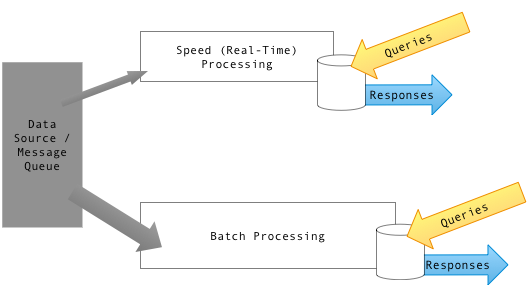
\includegraphics[width = 0.6\textwidth]{diagram_of_lambda_architecture.png}
    \caption[Architettura LAMBDA]{Diagramma di un'architettura LAMBDA \cite{lambdaArchitecture}}
\end{figure}

Il flusso elaborativo è esemplificato dai seguenti passi:
\begin{itemize}
    \item nella fase di \textit{ingestion}, i dati raw vengono catturati in modo simultaneo dalla sorgente. Questi dati alimentano un master dataset che funge da deposito immutabile e aggiornabile solo in modo incrementale, contenendo una copia inalterabile dei dati nel formato originale. Contestualmente, le componenti di processamento in \textit{streaming} vengono attivate per elaborare continuamente i dati in arrivo
    \item durante la fase di processamento, le componenti \textit{batch} intraprendono un approccio di ricalcolo totale o incrementale sul master dataset. Queste operazioni coinvolgono un alto volume di dati, presentano una latenza significativa e hanno un \textit{throughput} relativamente basso. Parallelamente, le componenti \textit{speed} processano lo stesso set di dati acquisito dalle operazioni \textit{batch}, fornendo risultati parziali attraverso tecniche di processamento real-time o pseudo real-time. Questo processo, eseguito a frequenze estremamente elevate e con bassa latenza, offre una visione istantanea e continua del blocco di dati trattato. I risultati ottenuti in questa fase vengono resi disponibili al \textit{Serving Layer}
    \item il \textit{Serving Layer}, infine, agisce come punto di convergenza, aggregando i risultati provenienti sia dalle operazioni \textit{batch} che da quelle in \textit{streaming}. Il suo ruolo principale è quello di fornire un'interfaccia unificata e coerente all'utente finale. Questo strato si occupa inoltre di sovrascrivere eventuali risultati parziali derivanti dall'elaborazione in \textit{streaming} con quelli ottenuti dalle operazioni \textit{batch}, garantendo così una visione complessiva e accurata dei dati trattati. Ad esempio, se nel processing in streaming vengono prodotti risultati parziali per un determinato set di dati, il \textit{Serving Layer} li integra con i risultati ottenuti dalle operazioni \textit{batch} per presentare all'utente una visione completa e aggiornata
\end{itemize}

Questo innovativo modello architetturale introduce notevoli elementi di cambiamento.
Innanzitutto, la mutabilità gestita tradizionalmente all'interno dei database enterprise viene sostituita dall'immutabilità del master dataset, il quale preserva la storia inalterata nel tempo nella sua forma originale.
Aggiunge continuamente nuovi flussi di dati senza mai rimuovere quelli precedenti.
I due strati si compensano reciprocamente in modo trasparente per gli utenti finali, offrendo una visione completa dei dati trattati.
Tale visione deriva da analisi approfondite sui dati storici e fornisce insight e statistiche parziali sui dati attuali.
Il master dataset persiste tipicamente utilizzando file system distribuiti (come \textit{Apache HDFS}) o database distribuiti \textit{NoSQL} (come \textit{MongoDB} orientato ai documenti, \textit{Redis} basato su chiavi, \textit{Neo4J} orientato ai grafi).
La combinazione di calcolo e storage parallelo distribuito consente di massimizzare il principio di località del dato.
Ciò implica il coordinamento e la distribuzione dell'elaborazione e del carico computazionale verso i nodi di lavoro che ospitano i blocchi di dati da elaborare.
Nel contesto di questa architettura, i principali framework di riferimento includono \textit{Apache Hadoop} \cite{hadoop} e \textit{Apache Spark} \cite{spark} per le componenti \textit{batch}, mentre per le componenti \textit{streaming} sono menzionati \textit{Apache Storm} e \textit{Spark Streaming}, che fa parte dell'ecosistema di \textit{Spark}.

\section[Stack SMACK]{Lo Stack SMACK}
La stack \textit{SMACK} è un insieme di tecnologie open source progettato per gestire e analizzare grandi volumi di dati in tempo reale.
L'acronimo \textit{SMACK} rappresenta le principali componenti dello stack: \textit{Spark}, \textit{Mesos}, \textit{Akka}, \textit{Cassandra} e \textit{Kafka}.
Ogni componente svolge un ruolo cruciale nel garantire una gestione efficiente, scalabile e resiliente dei dati.

\begin{figure}[!ht]
    \centering
    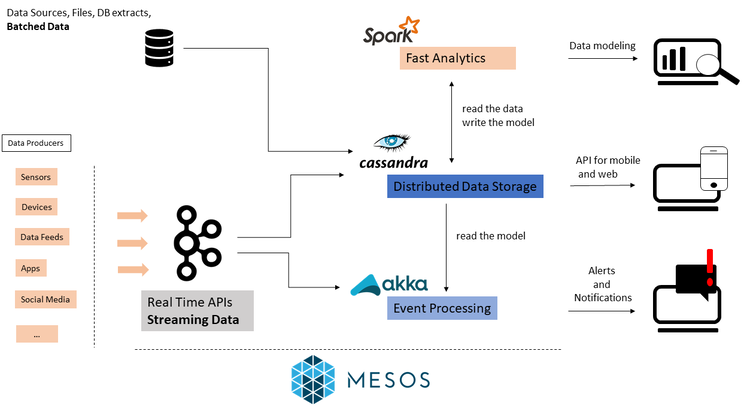
\includegraphics[width=0.6\textwidth]{smack.png}
    \caption[Stack SMACK]{Architettura dello Stack SMACK \cite{smack}}
\end{figure}

Analizziamo ogni componente:
\begin{itemize}
    \item \textbf{Apache Spark}: un framework di elaborazione distribuita che offre un modello di programmazione flessibile e veloce. 
    Spark facilita l'analisi di dati in tempo reale e fornisce un'interfaccia per il processing batch, streaming, SQL e machine learning. 
    La sua architettura a DAG (Directed Acyclic Graph) consente una pipeline di lavoro ottimizzata, promuovendo la velocità e la scalabilità.
    \begin{itemize}
        \item Modello di Programmazione Resiliente a Fallimenti (\textit{RDD}): Spark utilizza un modello di programmazione chiamato Resilient Distributed Dataset (\textit{RDD}). Gli \textit{RDD} sono collezioni distribuite di oggetti immutabili che possono essere elaborati in parallelo. Questo modello fornisce una gestione automatica dei fallimenti, consentendo a Spark di tollerare la perdita di dati durante l'elaborazione.
        \item \textit{Spark Core}: Questo è il nucleo del framework e fornisce le funzionalità di base di Spark, inclusa l'implementazione degli \textit{RDD} e l'engine di esecuzione distribuita. Spark Core è responsabile della gestione delle risorse, della tolleranza ai guasti e dell'interazione con lo storage distribuito.
        \item \textit{Spark SQL}: Questo modulo consente l'elaborazione di dati strutturati utilizzando SQL in Spark. Fornisce un'interfaccia per l'interrogazione dei dati attraverso comandi SQL standard, consentendo agli utenti di eseguire query su dati strutturati insieme alle elaborazioni batch e streaming.
        \item \textit{Spark Streaming}: È un modulo di Spark che consente l'elaborazione di dati in tempo reale. Utilizzando intervalli di microbatching, Spark Streaming elabora i dati in piccoli lotti, offrendo una soluzione per l'analisi dei dati in streaming senza dover ricorrere a un sistema separato.
        \item \textit{MLlib} (Machine Learning Library): Questa libreria integrata in Spark offre un'ampia gamma di algoritmi di machine learning scalabili. È progettata per semplificare lo sviluppo e l'implementazione di modelli di machine learning su grandi dataset distribuiti.
        \item \textit{GraphX}: È una libreria per l'elaborazione di grafi e l'analisi di dati basati su grafi. Grazie a GraphX, Spark può gestire in modo efficiente operazioni su grafi su scala distribuita, rendendolo adatto per applicazioni di social network, analisi delle reti, e altro ancora.
    \end{itemize}
    \item \textbf{Mesos} è un sistema di gestione delle risorse distribuite che fornisce un'astrazione delle risorse della macchina, consentendo l'esecuzione di applicazioni su cluster eterogenei. Mesos offre una gestione dinamica delle risorse, consentendo alle applicazioni di condividere efficientemente risorse come CPU e memoria, rendendo più flessibile l'utilizzo delle infrastrutture.
    
    \begin{figure}[h]
        \centering
        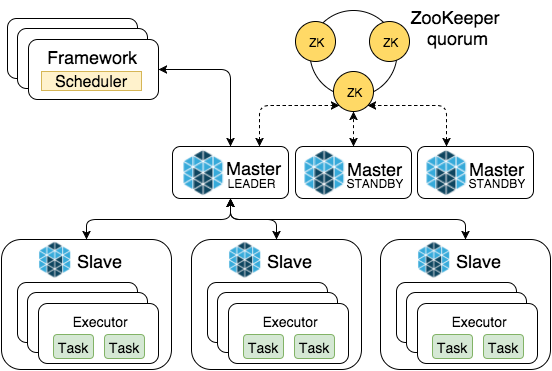
\includegraphics[width = 0.5\textwidth]{mesos.png}
        \caption[Architettura MESOS]{Diagramma dell'architettura di MESOS \cite{mesos}}
    \end{figure}

    \item \textbf{Akka} è un framework per la creazione di sistemi distribuiti e concorrenti basato sul modello di attori. Gli attori sono entità leggere che comunicano tra loro tramite messaggi, consentendo la costruzione di applicazioni altamente scalabili e resilienti. Akka facilita la gestione della concorrenza e fornisce strumenti per affrontare le sfide dei sistemi distribuiti.
    \item \textbf{Apache Cassandra} è un sistema di gestione del database distribuito altamente scalabile e altamente disponibile. Progettato per gestire grandi quantità di dati su cluster di macchine, Cassandra offre una distribuzione automatica dei dati e una replicazione multi-regionale, garantendo l'affidabilità e la resilienza del sistema anche in caso di guasti hardware o nodi inattivi.
    \item \textbf{Apache Kafka} è una piattaforma di streaming distribuito per la gestione di feed di dati in tempo reale. Kafka consente la pubblicazione e il consumo di eventi su larga scala, garantendo la robustezza e l'affidabilità delle pipeline di dati in tempo reale. La sua architettura a \textit{topic} consente una facile scalabilità e gestione dei flussi di dati.
\end{itemize}

Insieme, queste tecnologie formano la stack SMACK, offrendo una soluzione completa per l'elaborazione e l'analisi di dati in tempo reale su scala distribuita.
La combinazione sinergica di Spark, Mesos, Akka, Cassandra e Kafka fornisce un ambiente potente e flessibile per affrontare le sfide dell'analisi dei big data in tempo reale.

    \chapter[Programmazione ad Attori]{Attori: Scalabilità e Resilienza nel Modello di Programmazione}
    Il modello ad attori è un paradigma di programmazione concorrente che si basa sulla concettualizzazione di attori come unità di esecuzione indipendenti che comunicano tra loro attraverso lo scambio di messaggi. 
Questo approccio fornisce un modo efficace per gestire la concorrenza e costruire sistemi distribuiti altamente scalabili e resilienti. \\
L'uso del modello ad attori è motivato dalla necessità di semplificare lo sviluppo di applicazioni che richiedono un'elaborazione parallela efficiente. 
Invece di utilizzare tradizionali meccanismi di gestione della concorrenza come i thread, il modello ad attori permette agli sviluppatori di progettare applicazioni in cui attori indipendenti svolgono ruoli specifici e comunicano attraverso messaggi.
Questa modularità favorisce una progettazione più chiara e una gestione più agevole della complessità. \\
Inoltre, il modello ad attori promuove la scalabilità orizzontale, consentendo la distribuzione di attori su più nodi di un sistema distribuito o di un cluster.
Questa caratteristica è fondamentale per affrontare la crescente richiesta di elaborazione di grandi quantità di dati su ambienti distribuiti, fornendo una soluzione per costruire sistemi che possano crescere in modo flessibile in risposta ai carichi di lavoro. \\
La resilienza è un altro aspetto cruciale del modello ad attori.
Gli attori possono essere supervisionati da altri attori genitori, e in caso di fallimenti, il sistema può intraprendere azioni correttive come il ripristino dell'attore o l'adottare misure di compensazione.
Questo approccio contribuisce a costruire applicazioni robuste che possono gestire errori senza compromettere l'integrità dell'intero sistema.

\section[Concorrenza e parallelismo]{La differenza tra concorrenza e parallelismo}
Il parallelismo e la concorrenza sono concetti chiave nell'ambito dell'elaborazione e dell'esecuzione di task nei sistemi informatici.
Il parallelismo si riferisce all'esecuzione simultanea di più attività indipendenti allo scopo di migliorare l'efficienza complessiva del sistema.
In pratica, ciò implica la suddivisione di un problema in sotto-problemi indipendenti, che vengono eseguiti contemporaneamente da diverse unità di elaborazione. \\
D'altra parte, la concorrenza riguarda la gestione simultanea di più attività, ma non necessariamente in modo parallelo. 
Le attività concorrenti possono essere eseguite in momenti diversi e possono condividere risorse, richiedendo un meccanismo di coordinamento per evitare conflitti.
La concorrenza è spesso associata a sistemi multitasking, dove le attività vengono commutate rapidamente in modo apparentemente simultaneo, anche se in realtà vengono eseguite in modo alternato.

\begin{figure}[H]
    \centering
    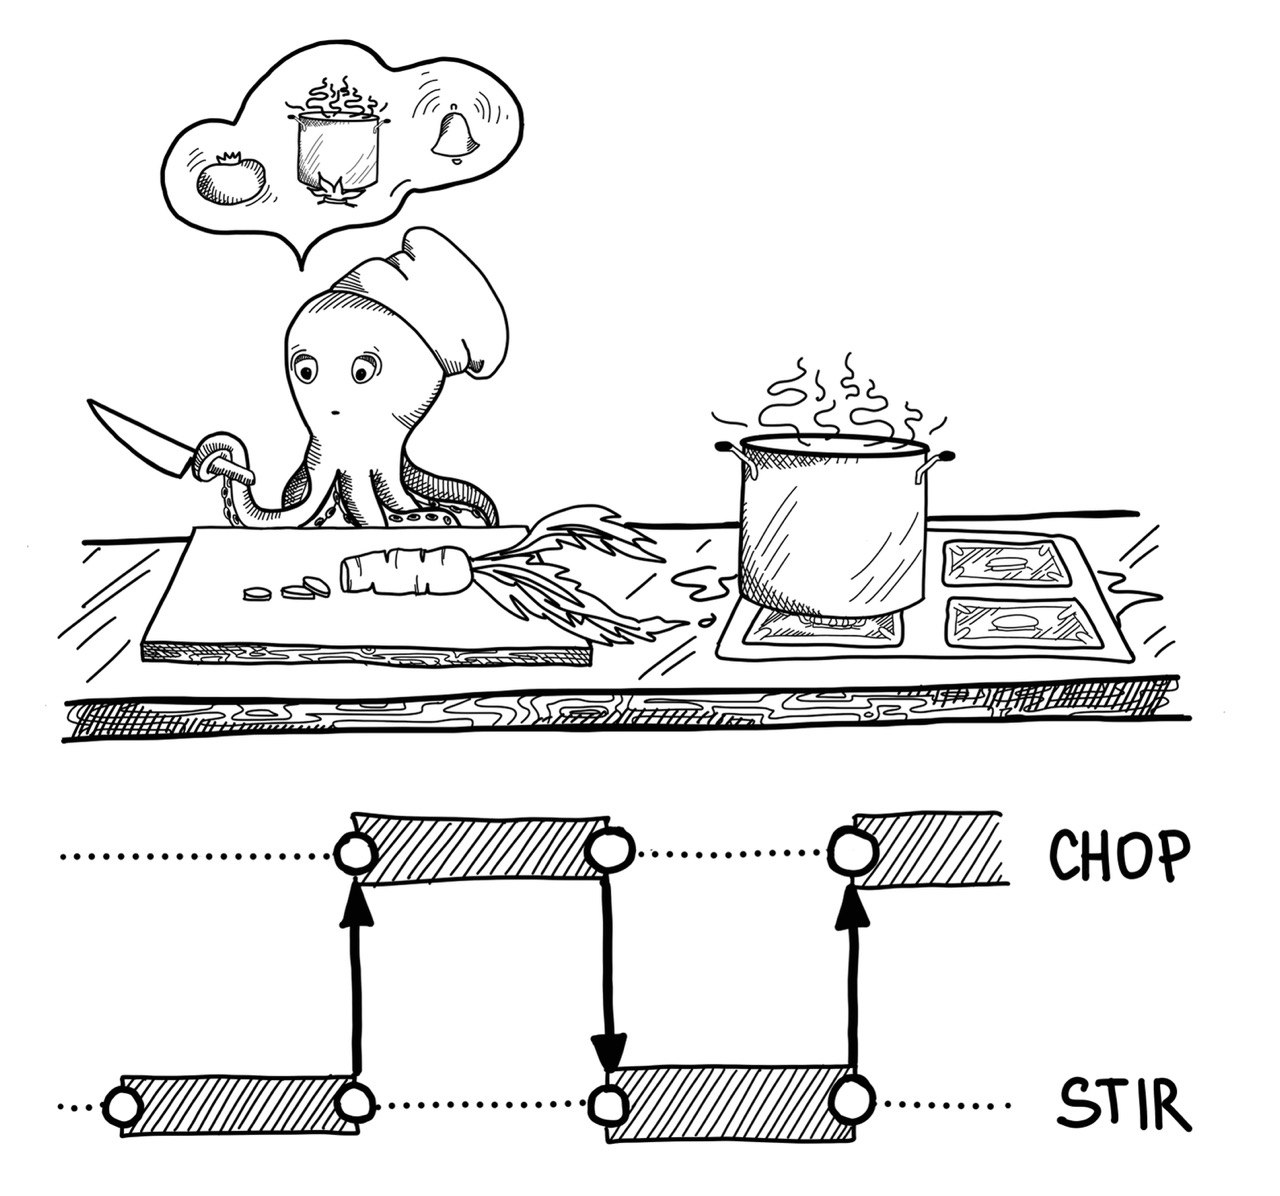
\includegraphics[width = 0.4\textwidth]{concurrency.jpg}
    \hspace{\fill}
    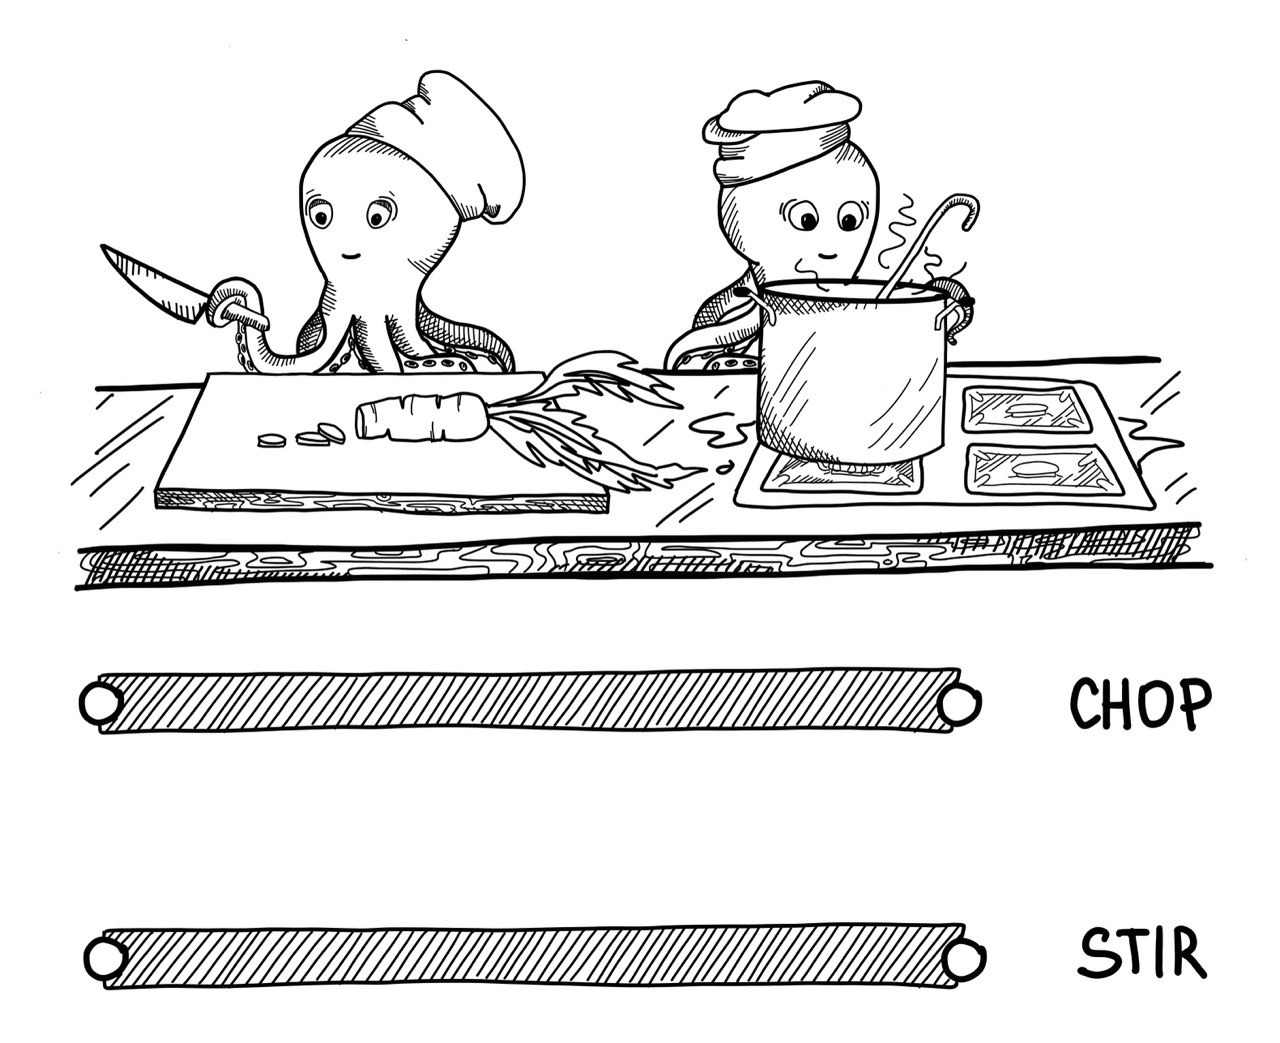
\includegraphics[width = 0.4\textwidth]{parallelism.jpg}
    \caption[Concorrenza e Parallelismo]{La differenza tra concorrenza e parallelismo \cite{parallelismConcurrency}}
\end{figure}

\section[Modello ad attori]{Il modello ad attori}
Il modello ad attori rappresenta un paradigma di programmazione che affonda le sue radici nelle teorie matematiche e nelle pratiche di elaborazione parallela. 
La sua storia si intreccia con il desiderio di affrontare le sfide emergenti dell'elaborazione parallela e distribuita. 
Un momento cruciale per la formulazione del modello ad attori fu l'opera "\textit{A universal modular ACTOR formalism for artificial intelligence}" \cite{actorsPaper} scritta da Carl Hewitt, Peter Bishop, e Richard Steiger nel 1973. 
Questo lavoro pionieristico introdusse i fondamenti teorici del modello ad attori, proponendo una visione innovativa dell'elaborazione parallela. \\
Il modello ad attori si basa sull'idea che l'unità fondamentale di elaborazione sia l'"attore", un'entità computazionale indipendente che comunica con gli altri attraverso lo scambio di messaggi.
Ogni attore è autonomo e possiede il proprio stato interno, eseguendo operazioni in risposta ai messaggi ricevuti.
Questo approccio decentralizzato favorisce la scalabilità e la gestione dell'elaborazione parallela. \\
Gli attori operano in modo asincrono, il che significa che possono procedere indipendentemente senza dover aspettare che altri attori completino le loro operazioni.
La comunicazione tra attori avviene esclusivamente tramite lo scambio di messaggi, e questo meccanismo di comunicazione definisce il flusso di controllo del programma. \\
Un aspetto distintivo del modello ad attori è la sua natura distribuita e la gestione della concorrenza.
Gli attori possono esistere e operare su sistemi distribuiti, consentendo un'elaborazione parallela su nodi separati.
La decentralizzazione offre una maggiore resistenza agli errori e una migliore tolleranza ai guasti, contribuendo a creare sistemi più robusti. \\
Negli anni successivi alla sua introduzione, il modello ad attori ha ispirato lo sviluppo di linguaggi di programmazione specifici, come Erlang, che implementano i principi fondamentali del modello ad attori.
Questi linguaggi sono stati utilizzati per la creazione di sistemi distribuiti, sistemi di telecomunicazione e applicazioni orientate agli eventi. \\

\begin{figure}[H]
  \centering
  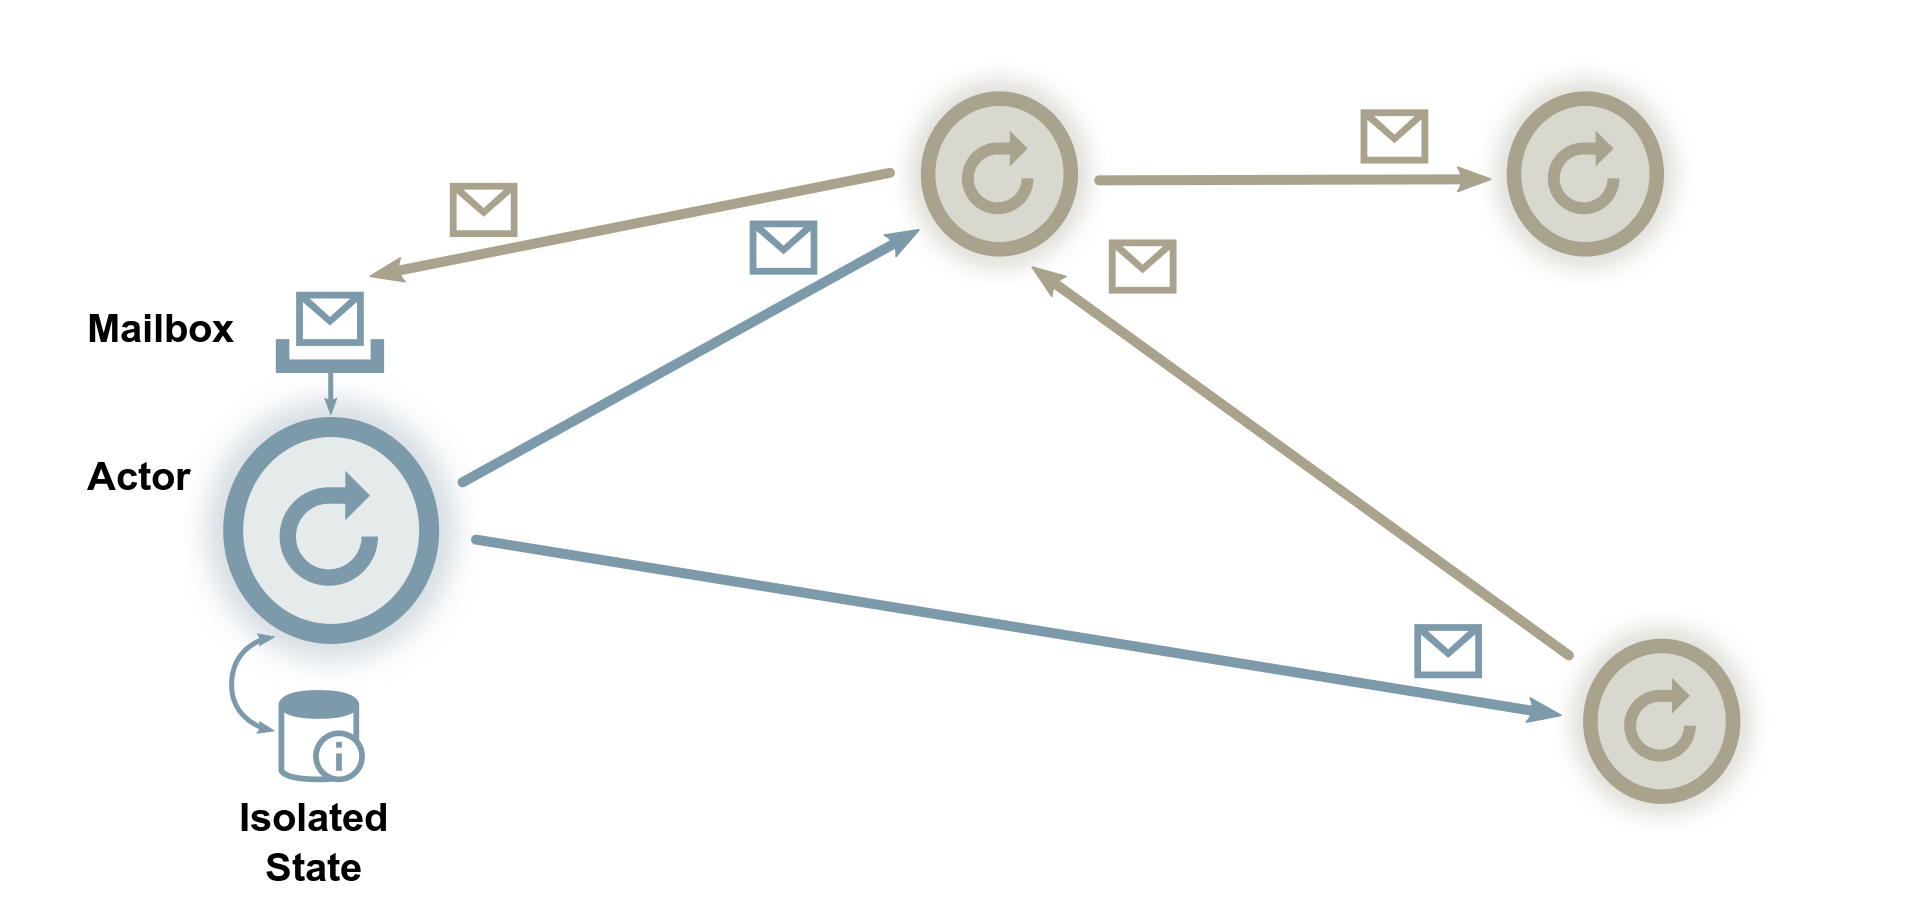
\includegraphics[width = 0.6\textwidth]{actors.png}
  \caption[Modello ad attori]{Modello ad attori \cite{actors}}
\end{figure}

Gli attori nel modello ad attori possiedono alcune caratteristiche chiave:
\begin{itemize}
    \item \textbf{Autonomia}: Ogni attore ha un proprio stato interno e un comportamento indipendente.
    Gli attori possono eseguire operazioni in modo asincrono, senza dover aspettare il completamento di altre attività.
    \item \textbf{Comunicazione tramite messaggi}: Gli attori interagiscono solo scambiandosi messaggi.
    Un attore può inviare un messaggio ad un altro attore, e questo scambio di messaggi costituisce il principale meccanismo di comunicazione nel modello.
    \item \textbf{Località e indirizzamento}: Gli attori possono esistere su sistemi distribuiti e hanno un indirizzo unico che li identifica.
    Questo consente agli attori di comunicare tra loro anche su reti distanti.
    \item \textbf{Isolamento dello stato}: L'isolamento dello stato significa che uno stato interno di un attore è accessibile solo da quell'attore specifico.
    Gli attori possono condividere informazioni solo scambiandosi messaggi, mantenendo così un livello di indipendenza.
    \item \textbf{Elaborazione di messaggi}: Gli attori eseguono operazioni in risposta ai messaggi che ricevono.
    Queste operazioni possono includere la modifica del proprio stato interno, l'invio di messaggi ad altri attori o la creazione di nuovi attori.
\end{itemize}

Sotto il profilo tecnico, un attore può essere considerato essenzialmente come un \textit{thread leggero}, ovvero un processo di esecuzione che è debolmente accoppiato con gli altri e si distingue per la sua capacità di inviare e ricevere messaggi.
Questo concetto è fondamentale nel contesto del modello ad attori, in cui l'interazione tra attori avviene attraverso il paradigma del message-passing. \\
L'invio e la ricezione di messaggi avvengono in modo asincrono, il che significa che il mittente non rimane bloccato in attesa di una risposta da parte del destinatario.
Questo approccio favorisce un'elaborazione parallela ed efficiente, consentendo agli attori di procedere con le proprie attività senza essere vincolati al completamento delle operazioni degli altri. \\
Ogni attore dispone di una coda di messaggi nota come \textit{mailbox}, dove i messaggi in arrivo vengono accodati in attesa di essere elaborati.
Il processo di elaborazione dei messaggi avviene secondo il principio \textit{FIFO} (\textit{First In First Out}), garantendo un ordine sequenziale nell'elaborazione.
Un singolo attore, inoltre, è in grado di processare un solo messaggio alla volta, il che contribuisce a mantenere l'ordine e la coerenza nell'esecuzione delle operazioni. \\
Un aspetto interessante è la possibilità di creare mailbox con priorità differenti per lo stesso attore, consentendo così un'ottimizzazione del processamento dei messaggi in base alla loro importanza relativa.
Questa caratteristica offre una maggiore flessibilità nell'implementazione di strategie di gestione dei messaggi, soprattutto quando si tratta di situazioni in cui alcuni messaggi potrebbero richiedere un'attenzione prioritaria rispetto ad altri. \\

Una regola fondamentale per garantire un efficace disaccoppiamento tra attori nel modello ad attori è il principio del \textit{tell-don't-ask} \cite{tellDontAsk}.
Questo principio sottolinea l'importanza di utilizzare chiamate asincrone non bloccanti per lo scambio di messaggi. \\
Nel contesto del modello ad attori, due modalità principali di comunicazione possono essere distinte:
\begin{itemize}
    \item \textbf{Fire-and-forget} (\textit{tell}): Consiste nell'invio di un messaggio senza attendere una risposta immediata.
    Eventuali risposte vengono ricevute attraverso la successiva ricezione di un nuovo messaggio al termine dell'azione richiesta.
    Questo approccio favorisce la non dipendenza da risposte immediate, contribuendo così a mantenere un flusso di esecuzione asincrono.
    \item \textbf{Request-response} (\textit{ask}): Questo approccio, più tradizionalmente adottato nelle applicazioni enterprise di tipo web, comporta l'invio di un messaggio sincrono seguito dall'attesa di una risposta.
    Tuttavia, è fortemente sconsigliato nel contesto delle applicazioni reattive poiché va in contrasto con i principi fondamentali di reattività.
    Inoltre, richiede un numero maggiore di thread per gestire le chiamate di callback, introducendo potenziali inefficienze nell'esecuzione.
\end{itemize}

In fase di creazione degli attori nel modello ad attori, è possibile definire gerarchie e strutturare una relazione padre-figlio, configurando così una struttura ad albero.
Questa organizzazione si rivela utile per automatizzare l'inoltro di nuovi messaggi verso i figli degli attori o per instradare messaggi in entrata.
In alternativa, gli attori possono fungere da \textit{guardiani}, supervisionando i loro figli e ricevendo notifiche in caso di malfunzionamenti.
Questa capacità di definire relazioni gerarchiche aggiunge un livello di organizzazione e controllo, contribuendo a una gestione più efficiente del sistema ad attori.

\section[Programmazione concorrente]{Programmazione concorrente}
La programmazione concorrente è un paradigma di programmazione che coinvolge l'esecuzione simultanea di più task o processi all'interno di un'applicazione.
Questa approccio è particolarmente utile per sfruttare al massimo le risorse di un sistema e migliorare le prestazioni complessive di un'applicazione.
Tuttavia, la programmazione concorrente presenta anche diverse criticità che devono essere gestite con attenzione.
Uno dei principali problemi è rappresentato dalle condizioni di gara, situazioni in cui più processi cercano di accedere o modificare una risorsa condivisa contemporaneamente, portando a risultati imprevedibili o errori.
La gestione della sincronizzazione diventa cruciale per evitare inconsistenze nei dati e problemi di accesso concorrente.
Altri aspetti critici includono la gestione dei \textit{deadlock}, situazioni in cui più processi sono bloccati perché ognuno attende che l'altro rilasci una risorsa, e la difficile individuazione e correzione degli errori dovuti alla concorrenza, che possono manifestarsi in modo sporadico e rendere complessa la fase di debugging.
Inoltre, la progettazione di algoritmi e strutture dati per la concorrenza richiede un'approfondita comprensione delle problematiche legate a questa modalità di esecuzione, rendendo la programmazione concorrente più complessa rispetto a quella sequenziale.

\begin{algorithm}[H]
    \SetKwInOut{Input}{Input}
    \SetKwInOut{Output}{Output}

    \Input{Amount $a$}
    \Output{$a$}
    \eIf{$deposit > a$}
      {
        $deposit \leftarrow (deposit - a)$ \\
        return $a$\;
      }
      {
        return $0$\;
      }
    \caption{Prelievo denaro da conto corrente}
\end{algorithm}

Cosa accade se due utenti chiamano contemporaneamente la funzione prelievo? Il primo utente potrebbe superare la verifica di disponibilità dell'importo prelevato dal conto, ma prima di effettuare l'effettivo prelievo, un secondo utente potrebbe anch'esso richiedere un prelievo, riducendo il saldo disponibile sul conto al di sotto dell'importo richiesto dal primo utente. 
Il risultato sarebbe un saldo negativo nel conto. 
Per affrontare questa situazione, se desideriamo implementare tale funzionalità in linguaggio C, con supporto alla concorrenza in un contesto \textit{multithreading} (dove ogni utente è un thread separato), sarebbe necessario utilizzare costrutti di sincronizzazione, come quelli forniti dalla libreria \textit{pthread}. \\
Questa soluzione potrebbe essere implementata bloccando l'intera attività di verifica e prelievo nella \textit{regione critica}, ma ciò comporterebbe un aumento della complessità nella codifica e un potenziale rischio di errori nell'implementazione.
Lo stesso si applicherebbe se dovessimo affrontare questa sfida utilizzando Java e sfruttando i costrutti di sincronizzazione forniti dalle API della \textit{JSE}. \\
Invece, mediante l'adozione del modello ad attori e l'utilizzo del toolkit Akka, l'intero processo verrà ricondotto a un'esecuzione atomica della funzione e allo scambio di messaggi per interagire con gli utenti. 
Il codice Scala per Akka appare notevolmente simile alla pseudo-codifica inizialmente presentata, con l'unica eccezione rappresentata dalla restituzione dell'output attraverso un messaggio.

\begin{algorithm}[H]
    \SetKwInOut{Input}{Input}

    \Input{Amount $a$}
    $value = 0$ \\
    \If{$deposit > a$}
      {
        $deposit \leftarrow (deposit - a)$ \\
        $value = deposit$;
      }
      $sender$ $!$ $gotCash(value)$
    \caption{Prelievo denaro da conto corrente con Scala e Akka}
\end{algorithm}

In merito alle sfide legate alla concorrenza, è importante considerare tre \textit{illusioni} comuni nel contesto delle soluzioni enterprise basate sul paradigma di programmazione orientato agli oggetti:
\begin{itemize}
    \item L'\textbf{incapsulamento} suggerisce che lo stato interno di un oggetto sia privato e accessibile solo tramite appositi metodi, noti come accessori e modificatori per la lettura e la scrittura rispettivamente.
    Questo approccio è efficace in contesti single-thread, ma mostra i suoi limiti in ambienti multi-thread.
    In tali scenari, le chiamate possono intrecciarsi in modo non deterministico, compromettendo la possibilità di garantire una sequenza predefinita di esecuzione, a meno che non si ricorra nuovamente a meccanismi di sincronizzazione.
    \item La \textbf{gestione della memoria condivisa} in architetture multi-core presenta sfide significative. Le moderne architetture dei computer incorporano più unità di calcolo, ognuna con la propria memoria cache a livello CPU, non visibile alle altre.
    Questo può portare a inconsistenze tra i thread appartenenti a core diversi che manipolano lo stesso oggetto memorizzato nelle rispettive cache.
    L'unico rimedio è la sincronizzazione delle cache.
    Alcuni linguaggi offrono direttive per istruire il processore a recuperare un oggetto esclusivamente dalla memoria principale, evitando l'utilizzo delle cache delle CPU.
    Ad esempio, in Java, la keyword \textit{volatile} può essere utilizzata per definire un attributo di una classe e renderlo \textit{thread-safe}.
    \item L'esecuzione di \textbf{task in background} è comune in quasi tutti i linguaggi di programmazione, consentendo la specifica di un riferimento a cui richiamare una funzione al termine dell'esecuzione.
    Tuttavia, si presenta una problematica quando il thread incaricato di eseguire il task incontra un errore.
    In questo caso, il thread non dispone di mezzi per comunicare con il thread chiamante e notificare l'errore, poiché il call stack sarà inutilizzabile a seguito dell'eccezione.
    Questa situazione può rendere difficile la gestione degli errori nei task in background.
\end{itemize}

Il modello ad attori si propone di affrontare le sfide associate alla concorrenza e alla distribuzione di codice attraverso l'implementazione di poche e chiare regole:
\begin{itemize}
  \item \textbf{Comunicazione Asincrona Esclusiva}: il modello ad attori adotta un approccio di scambio asincrono di messaggi come unico mezzo di comunicazione tra attori.
  Questa scelta impedisce situazioni di blocco incontrollato, consentendo l'esecuzione atomica e deterministica delle istruzioni contenute nel codice della funzione.
  Ciò garantisce la coerenza dello stato incapsulato nell'oggetto.
  \item \textbf{Elaborazione FIFO} (\textit{First-In-First-Out}): gli attori gestiscono i messaggi in arrivo secondo il principio FIFO, assicurando che i messaggi vengano elaborati nell'ordine in cui sono stati ricevuti nella coda dell'attore.
  \item \textbf{Stato Locale e Non Condiviso}: lo stato degli attori è locale e non condiviso, comunicato esclusivamente attraverso lo scambio di messaggi.
  Questo approccio favorisce l'isolamento e la coerenza dei dati tra gli attori.
  \item \textbf{Gestione delle Eccezioni}: il modello ad attori gestisce le eccezioni in modo da notificare al chiamante eventuali fallimenti tramite un messaggio di risposta.
  Questa pratica contribuisce a una gestione robusta degli errori nel contesto della concorrenza distribuita.
  \item \textbf{Tecniche di Supervisione}: vengono adottate tecniche di supervisione per monitorare il comportamento degli attori e decidere l'azione appropriata in risposta a eventuali fallimenti di un attore.
  Questa capacità di supervisione migliora la resilienza del sistema distribuito.
\end{itemize}
In sintesi, l'applicazione di queste regole e l'adesione a pratiche consigliate consentono lo sviluppo di codice concorrente distribuito sicuro.
Va notato che, sebbene il modello ad attori non possa garantire lo stesso livello di parallelizzazione delle applicazioni native multithread, fornisce comunque strumenti per rendere il sistema scalabile.
L'adozione di queste regole semplifica la gestione della concorrenza e della distribuzione, contribuendo a una progettazione più affidabile e resiliente del software.

\section[Cassetta degli attrezzi]{La cassetta degli attrezzi}
Esaminiamo adesso l'approccio di Akka come framework per realizzare il paradigma degli attori all'interno delle nostre soluzioni, avvalendoci del linguaggio di programmazione Scala. Questo linguaggio, per la sua intrinseca natura funzionale, si dimostra particolarmente idoneo in situazioni in cui la scalabilità è un requisito essenziale.

\subsection[SCALA]{Il linguaggio di programmazione SCALA}
Il termine \textit{Scala} è una contrazione di SCAlable LAnguage ed è stato coniato nel 2001 presso la Scuola Politecnica Federale di Losanna, in Svizzera, da Martin Odersky, l'attuale fondatore di Lightbend.
Quest'azienda si occupa del monitoraggio degli sviluppi del linguaggio, della formazione e della consulenza professionale. \\
Scala si posiziona all'incrocio della programmazione funzionale, della programmazione ad oggetti e dei linguaggi di scripting.
Questa peculiarità deriva dalla sua capacità di offrire i costrutti tipici della programmazione funzionale, i principi e le regole della programmazione ad oggetti, consentendo nel contempo un prototipaggio rapido grazie al linguaggio conciso che lo assimila a linguaggi di scripting tradizionali. \\
Il linguaggio è particolarmente adatto per la scrittura di codice scalabile, basandosi su concetti chiave come l'immutabilità dei dati, il passaggio di funzioni e la valutazione pigra delle istruzioni. \\
Durante la compilazione, il codice Scala genera bytecode Java, che viene interpretato ed eseguito dalla \textit{Java Virtual Machine} (JVM).
Ciò rende Scala completamente interoperabile con il codice scritto in Java o altri linguaggi che generano bytecode Java, offrendo un evidente vantaggio nel riutilizzo di librerie già esistenti. 

\begin{figure}[H]
  \centering
  
\includegraphics[width = 0.2\textwidth]{scala_logo.png}
  \caption[SCALA Logo]{Il logo del linguaggio SCALA \cite{scala}}
\end{figure}

Le caratteristiche distintive del linguaggio Scala comprendono:
\begin{itemize}
  \item \textbf{Funzioni di Prima Classe}: Questa caratteristica, ereditata dai linguaggi funzionali, consente alle funzioni di essere trattate come variabili.
  Possono essere assegnate a variabili e passate come argomenti a altre funzioni.
  Questo paradigma offre una flessibilità notevole nel design del software, facilitando la creazione di codice modulare e riutilizzabile.
  \item \textbf{Inferenza dei Tipi}: Scala presenta un sistema di inferenza dei tipi che elimina la necessità di dichiarare esplicitamente il tipo di una variabile.
  Il tipo può essere dedotto automaticamente durante la valutazione dell'espressione.
  Questo aspetto semplifica il processo di scrittura del codice, rendendo Scala particolarmente adatto per attività di prototipazione rapida, riducendo il costo di progettazione del software e consentendo una maggiore operatività immediata.
  \item \textbf{Funzioni Anonime}: Trattando le funzioni come oggetti, Scala permette la definizione di funzioni anonime in-line.
  Questo significa che è possibile implementare una funzione specificando solo il corpo, l'input e l'output dell'implementazione senza dover dichiarare staticamente la funzione.
  Questa flessibilità è utile per semplificare la scrittura del codice e migliorare la leggibilità.
  \item \textbf{Valutazione Pigra}: Scala adotta la valutazione pigra, che ritarda l'esecuzione delle espressioni fino al momento in cui i valori ottenuti sono effettivamente necessari.
  Questo approccio contribuisce all'efficienza del programma, evitando la valutazione di espressioni superflue e ottimizzando l'utilizzo delle risorse.
  \item \textbf{Pattern Matching}: Oltre a esaminare il valore in sé, Scala consente il pattern matching, che comporta la verifica di modelli di scomposizione del valore in diverse parti.
  Questa caratteristica si rivela particolarmente potente nell'implementazione di logiche complesse e nella gestione di strutture dati intricate.
  \item \textbf{Immutabilità}: Per promuovere la scalabilità e la sicurezza in contesti concorrenti, Scala incoraggia l'uso di valori immutabili.
  Questo significa che, una volta definito un valore, non può essere modificato.
  Tale pratica riduce il rischio di inconsistenze causate da variabili mutevoli, contribuendo a una progettazione del software robusta e thread-safe.
  \item \textbf{Utilizzo di Tuple}: Scala offre il supporto per le tuple, che sono strutture dati immutabili contenenti un numero fissato di elementi, ognuno con un proprio tipo distinto.
  Le tuple sono utili per rappresentare collezioni eterogenee di dati in modo conciso ed efficiente.
  \item \textbf{Orientamento Completo agli Oggetti}: A differenza di alcuni linguaggi come Java, Scala è completamente orientato agli oggetti.
  Ogni elemento, che siano funzioni, letterali stringa o numeri, è definito e trattato come un oggetto.
  Questa coerenza nella progettazione del linguaggio semplifica la comprensione e la gestione del codice.
\end{itemize}

\subsection[AKKA]{Ambiente AKKA}
Come precedentemente enunciato, Akka rappresenta un toolkit ideato da Jonas Bonér all'interno della società Typesafe, ora denominata Lightbend, di cui Bonér è cofondatore insieme al creatore di Scala, Martin Odersky.
Questa piattaforma consente la progettazione di programmi che operano in modo parallelo e concorrente, aderendo al modello ad attori.
Ciò viene realizzato senza richiedere al programmatore la conoscenza dettagliata e l'impegno richiesto nella risoluzione delle comuni problematiche che emergono nei sistemi concorrenti.
Tali sfide vanno dalla gestione low-level di processi e thread fino alla sincronizzazione, affrontando fenomeni come deadlock, starvation e race condition.
L'obiettivo chiave di Akka è di assistere il programmatore nell'implementazione di soluzioni parallele, asincrone, altamente scalabili e resilienti.
Merita rilevare che Akka è interamente implementato utilizzando il linguaggio Scala. \\
Akka sposa la filosofia di Carl Hewitt e del suo modello ad attori, concependo l'attore come l'unità primitiva e universale di elaborazione per la programmazione concorrente.
Hewitt, con grande lungimiranza, progettò questo modello con l'anticipazione di un ambiente in cui l'elevata parallelizzazione fosse resa possibile dall'uso su larga scala di microprocessori indipendenti e geograficamente distribuiti, capaci di comunicare a basse latenze.
Questa visione di Hewitt è diventata ora una realtà con l'avvento del Cloud Computing, e Akka è stato appositamente concepito per adottare e implementare tali principi. \\
Adesso, procederemo all'analisi approfondita delle caratteristiche principali di Akka. 
Esploreremo il livello di astrazione fornito per la programmazione concorrente, il meccanismo di comunicazione basato sul passaggio di messaggi, l'utilizzo di processi leggeri, il ciclo di vita degli attori, la capacità di auto-ripristino (self-healing), la trasparenza della localizzazione, il routing dei messaggi e l'implementazione del clustering per soddisfare i requisiti di scalabilità.

\begin{figure}[H]
  \centering
  
\includegraphics[width = 0.2\textwidth]{akka_logo.png}
  \caption[Logo AKKA]{Il logo del toolkit AKKA \cite{akka}}
\end{figure}

\subsubsection[Programmazione concorrente]{Livello di atrazione per la programazione concorrente}
L'entità attoriale, ritenuta l'elemento cardine per il computo, la conservazione e la trasmissione di informazioni, si distingue per la sua prudenza nell'evitare di esporre il proprio stato interno.
La comunicazione tra attori avviene mediante lo scambio di messaggi, che sono \textit{immutabili}, \textit{asincroni} e \textit{non vincolanti}.
Questa strategia consente una flessibilità e una scalabilità notevoli nel contesto di sistemi concorrenti.
L'attore, come unità primitiva, attua la sua logica di business in risposta agli stimoli esterni che gli vengono trasmessi tramite messaggi.
Tuttavia, è importante sottolineare che le operazioni consentite da un attore sono limitate al modello ad attori, il che implica la possibilità di inviare messaggi, creare nuovi attori e definire comportamenti interni in risposta a specifici messaggi. \\
L'impiego di messaggi immutabili è una scelta progettuale intrinseca, concepita per mitigare possibili problematiche di concorrenza e inconsistenza di stato.
Questa caratteristica assicura che attori distinti, nel medesimo istante temporale, visualizzino versioni consistenti e uniformi dello stato di un attore.
Ciò contribuisce in modo significativo all'integrità e alla coerenza del sistema, mitigando gli effetti indesiderati che potrebbero emergere in scenari concorrenti complessi. \\
Esaminiamo ora il processo di definizione di un attore, con particolare riferimento agli esempi che seguiranno, tutti redatti in linguaggio Scala.
A tale scopo, delineeremo l'evoluzione di un programma \textit{Hello World}, un esercizio storico spesso adoperato per illustrare i concetti basilari di sintassi e funzionamento.
Questa scelta ci consentirà di analizzare in dettaglio come il linguaggio Scala si integri e si adatti al paradigma ad attori in questo specifico contesto. 

\lstinputlisting[language=Scala, float=ht]{code/HelloWorldActor.java} 

All'interno del caso pratico illustrato, l'entità denominata \textit{Greeter} assume il compito di accogliere un nome specifico e di renderlo visibile attraverso la stampa su dispositivo video.
Questo processo di trasmissione di informazioni è mediato da un messaggio immutabile, precisamente delineato dalla struttura definita nella classe Greet. \\
Per approfondire questo concetto, è rilevante esaminare in dettaglio la dinamica sottostante.
In questo contesto, la classe \textit{Greeter} non è solo un semplice oggetto che riceve e stampa un nome; essa incarna un attore all'interno del modello ad attori.
L'adozione del paradigma ad attori consente una gestione asincrona ed efficiente degli stimoli esterni, in questo caso, rappresentati dalla ricezione di messaggi immutabili. \\
La scelta di utilizzare un messaggio immutabile, come definito dalla classe Greet, è una decisione progettuale strategica.
Tale struttura immutabile, per sua natura, contribuisce a prevenire problematiche legate alla concorrenza e alla consistenza dello stato.
Inoltre, essa riflette il principio fondamentale dell'immutabilità nell'ambito del modello ad attori, dove ogni messaggio rappresenta un'istanza unica e indipendente di dati. \\
In questo scenario, la comunicazione tra attori, manifestata attraverso il passaggio di messaggi, sottolinea l'approccio decentralizzato e distribuito del modello ad attori.
Questo design non solo favorisce la modularità del sistema, ma anche la creazione di un ambiente altamente scalabile e reattivo. \\
Per cogliere appieno la complessità e la potenza di questo approccio, è utile analizzare ulteriori aspetti relativi alla gestione degli attori, alla definizione di comportamenti in risposta a messaggi specifici e alla gestione del ciclo di vita dell'attore stesso.
In questo modo, possiamo apprezzare l'efficacia e la versatilità del paradigma ad attori nell'implementazione di soluzioni software resilienti, parallele e altamente scalabili. 

\lstinputlisting[language=Scala, float=ht]{code/App.java} 

Affinché l'intero processo venga avviato, è necessario inizializzare l'ambiente creando il sistema, procedendo all'istanziazione del nuovo attore attraverso l'utilizzo del metodo di fabbrica (\textit{factory method}) denominato \textit{props} e, successivamente, inoltrare un messaggio asincrono e non bloccante alla classe chiamante. \\

Per esplorare più approfonditamente questa sequenza di operazioni, è vantaggioso considerare i dettagli operativi di ciascuna fase. 
In primo luogo, la creazione del sistema costituisce un passaggio cruciale. In questo contesto, \textit{system} rappresenta il quadro globale entro il quale gli attori interagiscono, e la sua istanziazione stabilisce l'ambiente di esecuzione in cui gli attori agiscono.
Successivamente, l'azione di istanziare un nuovo attore mediante il metodo \textit{props} introduce la flessibilità e la configurabilità nell'ambito della creazione degli attori.
Questo metodo, funzionando come una sorta di fabbrica, accetta i parametri necessari per definire il comportamento e le caratteristiche dell'attore in questione.
Tale approccio favorisce la modularità e la personalizzazione nell'implementazione degli attori, rendendo possibile la creazione di diverse istanze con comportamenti specifici. \\
L'invio di un messaggio asincrono e non bloccante alla classe chiamante costituisce l'ulteriore passo in questa sequenza operativa.
Questo processo di comunicazione asincrona permette alla classe chiamante di proseguire la sua esecuzione senza dover attendere una risposta immediata dall'attore appena creato.
Tale aspetto è cruciale in un contesto di programmazione concorrente, in quanto consente alle attività di procedere in modo parallelo, migliorando l'efficienza e la reattività del sistema nel suo complesso. \\
Inoltre, è interessante notare come la scelta di un messaggio non bloccante contribuisca alla fluidità e alla dinamica del flusso di esecuzione complessivo.
Questo approccio consente di evitare situazioni in cui la classe chiamante si bloccherebbe in attesa di una risposta sincrona, mantenendo invece la continuità delle operazioni in modo agile e responsivo.

\subsubsection[Comunicazione]{La comunicazione tra Attori}
Akka concepisce la definizione di un attore in modo simile a una struttura dell'object-oriented, ma si distingue notevolmente in quanto non espone alcun metodo o attributo direttamente.
L'interazione con un attore avviene esclusivamente attraverso l'invio di messaggi, un paradigma di comunicazione event-driven implementato mediante il \textit{message passing}.
Ogni attore è dotato di un proprio buffer denominato \textit{mail-box}, una sorta di casella di posta, dove i messaggi vengono accodati e successivamente estratti in modo sincrono e bloccante, seguendo l'ordine di ricezione (\textit{First-In-First-Out}).
Ogni messaggio è associato a un thread specifico per l'elaborazione.
Va notato che non esiste una garanzia assoluta di recapito corretto dei messaggi.
Nel caso in cui la consegna fallisca, il messaggio viene instradato verso una mail-box di sistema denominata \textit{dead letters}. \\
In un contesto asincrono, se, ad esempio, gli attori A e B inviano messaggi all'attore C in successione, non c'è certezza che i messaggi saranno ricevuti nel medesimo ordine di invio.
La sola garanzia fornita dal sistema è che, all'interno di una coppia mittente/destinatario specifica, i messaggi saranno elaborati dal destinatario nell'ordine di invio. \\
Gli attori possono comunicare tra loro mediante azioni di \textit{tell} o \textit{ask}, rispettivamente utilizzate per comunicazioni di tipo \textit{fire-and-forget} o \textit{request-response}.
Tuttavia, al fine di mantenere i principi di disaccoppiamento, è fortemente scoraggiato lo scambio di messaggi bloccanti di tipo \textit{ask}.
Tale pratica è considerata una violazione dei principi fondamentali del modello ad attori, poiché compromette la scalabilità, favorendo invece l'utilizzo del tipo \textit{tell}. \\
Questa configurazione specifica del modello ad attori enfatizza la natura asincrona delle interazioni, incoraggiando un design che favorisca la modularità, la reattività e la scalabilità all'interno dei sistemi che adottano Akka.
La comprensione approfondita di queste dinamiche consente di sfruttare al massimo i benefici offerti dal paradigma ad attori nella costruzione di applicazioni robuste e altamente performanti. 

\begin{figure}[H]
  \centering
  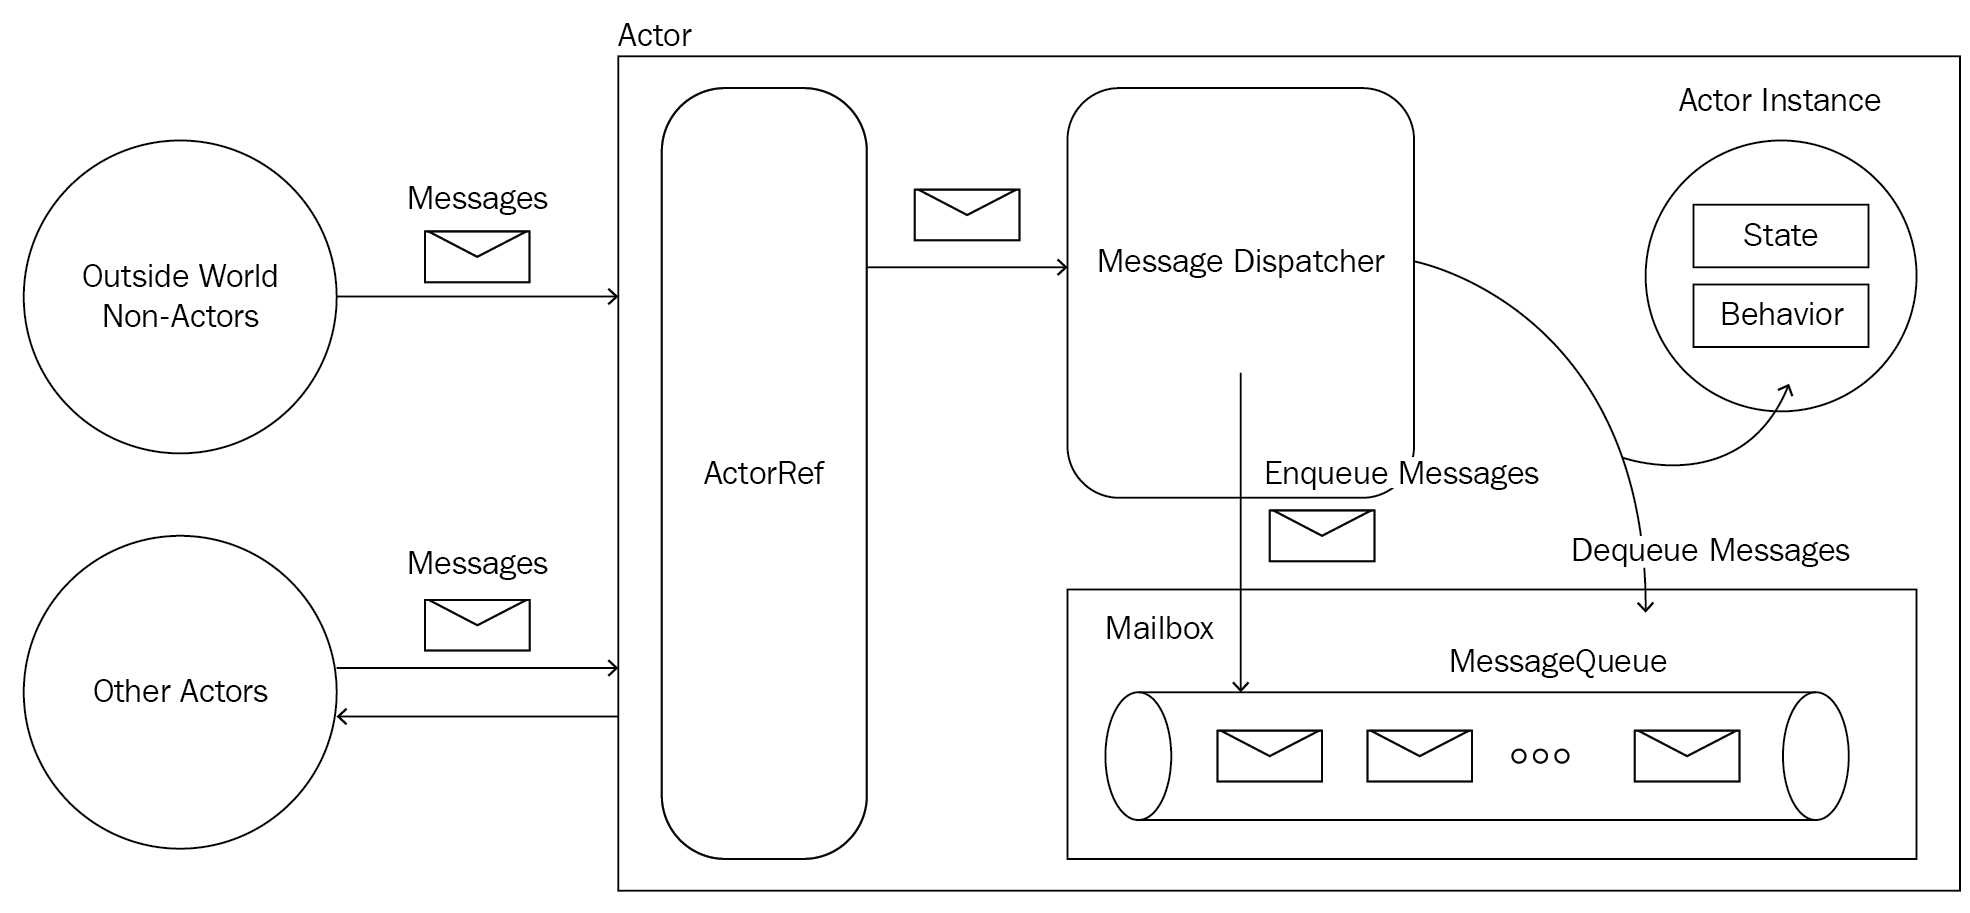
\includegraphics[width = 0.95\textwidth]{akka_messages.png}
  \caption[Componenti AKKA]{Diagramma delle componenti interni di un Attore e come interagiscono tra di loro}
\end{figure}

Esempio di un invio di messaggio asincrono \textit{fire-and-forget}:

\begin{lstlisting}
  greeter ! Greet("Elon");
\end{lstlisting}

Invio messaggio sincrono \textit{request}/\textit{response}, con gestione attesa valore di ritorno mediante costrutto \textit{Future}:

\lstinputlisting[language=Scala, float=ht]{code/Future.java} 

L'attore, in questa configurazione specifica, abbandona la pratica di stampare il messaggio a video, invece opta per restituirlo al chiamante.
Nel corso di questa operazione, il chiamante si troverà in uno stato di blocco in attesa della risposta.
Questo comportamento è dettato dall'impiego dell'operatore "?" (\textit{ask}) anziché "!" (\textit{tell}) per l'invio del messaggio. \\
È di rilievo esplorare più a fondo il concetto di \textit{ask pattern}.
Questa scelta determina una variante nel paradigma di recapito del messaggio noto come \textit{at-most-once}.
Tale paradigma offre la garanzia che la consegna del messaggio avvenga al massimo una sola volta, ma non fornisce alcuna assicurazione sull'effettiva avvenuta consegna. \\
È cruciale comprendere le differenze con il paradigma \textit{at-least-once}, il quale garantisce l'effettiva consegna del messaggio ma non impedisce che il messaggio venga recapitato più volte.
Un altro paradigma, denominato \textit{exactly-once}, offre la certezza che la consegna si verifichi una e una sola volta. \\
Akka, coerentemente con i principi fondamentali del modello ad attori, adotta il paradigma \textit{at-most-once}.
Questa scelta strategica è orientata a evitare l'introduzione di complessità nella codifica e di overhead prestazionali.
Il sistema sfrutta la capacità di supervisione degli attori per gestire eventuali fallimenti, una caratteristica intrinseca del modello ad attori.
In contrasto, un approccio \textit{at-least-once} richiederebbe l'implementazione di un protocollo personalizzato per la gestione di \textit{ACK/NACK}, al fine di ottenere feedback sulla consegna.
Analogamente, un approccio \textit{exactly-once} implicherebbe l'implementazione di logiche complesse per garantire la consegna e scartare eventuali messaggi duplicati.
Questa riflessione sottolinea l'acume di Akka nel bilanciare la garanzia di consegna dei messaggi con l'obiettivo di mantenere un approccio snello e performante, integrando al contempo la capacità di gestire dinamicamente eventuali fallimenti all'interno dell'ecosistema ad attori.

\subsubsection[Ciclo di vita]{Ciclo di vita degli attori}
Il percorso evolutivo di un attore è caratterizzato da tre differenti categorie di eventi, ognuna delle quali assume un ruolo significativo nella gestione dinamica dell'entità attoriale:
\begin{itemize}
  \item \textbf{Creazione dell'Attore} (Stato: \textit{Started}): la fase iniziale è rappresentata dalla creazione dell'attore, la quale lo colloca nello stato di \textit{started}.
  La generazione di un attore avviene mediante l'applicazione del metodo \textit{actorOf} sul \textit{actorSystem}.
  Questo processo inaugura la vita dell'attore, preparandolo per le interazioni e le responsabilità che andrà ad assumere nel corso del suo ciclo di vita.
  \item \textbf{Riavvio dell'Attore} (\textit{Strategia di Supervisione}): un evento cruciale si verifica quando un attore affronta un fallimento e si attiva la strategia di supervisione.
  In questo contesto, il riavvio dell'attore è innescato su richiesta del supervisore, il quale, con saggezza, decide di riportare in vita l'attore.
  Tale processo di riavvio implica l'esecuzione di hook specifici, come \textit{preRestart} e \textit{postRestart}, permettendo l'iniezione di eventuali segmenti di codice aggiuntivo durante queste fasi critiche.
  Questo approccio flessibile consente di gestire dinamicamente i fallimenti e di reintegrare l'attore nella sua operatività con le correzioni necessarie.
  \item \textbf{Terminazione dell'Attore} (Stato: \textit{Stopped}): la fase di stop segna la conclusione dell'operatività dell'attore, trasferendolo nello stato di \textit{stopped}.
  Questa terminazione può essere avviata sia dal supervisore che dall'attore stesso.
  Una volta in questo stato, i successivi messaggi indirizzati all'attore verranno instradati verso la mail-box di sistema denominata \textit{dead letters}.
  È rilevante notare che nello scenario di default, lo stop di un attore comporta la cessazione delle attività anche per tutti i suoi attori figli.
\end{itemize}
Esaminando attentamente ciascuna di queste fasi, emergono le dinamiche complesse e le considerazioni strategiche che permeano il ciclo di vita di un attore all'interno di un sistema basato su Akka.
Questa prospettiva dettagliata fornisce una panoramica esaustiva delle diverse transizioni e delle opportunità per gestire eventuali problematiche, sottolineando l'elasticità e la robustezza insite nell'approccio ad attori implementato da Akka.

\subsubsection[Processo leggero]{Processo leggero}
Nel contesto di Akka, ciascun attore si manifesta come un processo leggero, denominato \textit{light}, il che consente una notevole agilità esecutiva, con un'approssimativa capacità di gestire fino a 2.7 milioni di attori per ogni gigabyte di memoria RAM.
L'orchestrazione di questo scenario avviene quando un attore, ricevendo un messaggio nella propria mail-box, si impegna nel processo di elaborazione grazie a un thread assegnatogli dal componente \textit{Dispatcher}.
La gestione dell'aspetto multi-threaded è strategicamente attuata all'interno di questo componente, evidenziando la robustezza e la scalabilità del toolkit.

Akka offre nativamente diverse opzioni di dispatcher, ciascuna progettata per adattarsi a specifiche esigenze di gestione dei thread. Tra queste opzioni, troviamo:
\begin{itemize}
  \item \textit{SimpleDispatcher}: frutta i thread-pool per condividere l'uso di thread tra attori diversi.
  Questa strategia si rivela particolarmente utile nel contesto di un sistema in cui la condivisione di risorse è una priorità, consentendo un'efficace gestione dell'allocazione di thread tra attori distinti.
  \item \textit{PinnedDispatcher}: assegna un thread dedicato a ciascun attore, promuovendo un'approccio più isolato e specifico per la gestione di ogni entità attoriale.
  Questa configurazione è vantaggiosa in situazioni in cui è necessaria una separazione marcata tra le attività degli attori.
  \item \textit{CallingThreadDispatcher}: esegue più invocazioni riutilizzando lo stesso thread, una scelta solitamente riservata a scopi di debug.
  Questa opzione permette di semplificare il tracciamento e la comprensione delle chiamate, facilitando le operazioni di debugging.
\end{itemize}
L'implementazione di queste strategie di dispatcher consente di ottimizzare l'allocazione e l'utilizzo dei thread in modo flessibile, consentendo a ogni attore di sfruttare efficientemente le risorse disponibili.
Questo approccio, in cui il numero di attori allocabili per unità di memoria supera ampiamente il numero di thread istanziabili, sottolinea l'efficienza e la scalabilità della progettazione di Akka, contribuendo così a costruire sistemi altamente reattivi e performanti.

\subsubsection[Fault tolerance]{Fault tolerance}
Esaminiamo con attenzione l'approccio di Akka alla gestione della \textit{fault tolerance}, un aspetto cruciale per garantire la robustezza e l'affidabilità dei sistemi attoriali.
Durante il processo di creazione degli attori, emerge la possibilità di definire una gerarchia, consentendo di stabilire se l'attore appena creato instaurerà una relazione padre-figlio o discenderà direttamente dalla radice del sistema.
Questa scelta innesca la formazione di una relazione di supervisione, la cui dinamica può essere plasmata attraverso l'adozione di specifiche strategie, sia personalizzate che fornite nativamente dal toolkit. \\
All'inizio del ciclo vitale del sistema attoriale, si delineano tre attori radice: il \textit{root guardian}, che rappresenta la radice effettiva dell'albero gerarchico; lo \textit{user guardian}, padre di tutti gli attori dell'applicazione; e il \textit{system guardian}, responsabile della supervisione degli attori di sistema. \\
Ad esempio, in caso di insuccesso di un attore figlio, il supervisore può intraprendere diverse azioni, tra cui il riavvio, la terminazione o la delega del problema al proprio supervisore.
Questo paradigma, noto come \textit{let it crash}, si distingue per la scelta di consentire il fallimento dell'attore supervisionato anziché implementare complesse logiche di gestione delle eccezioni.
In questo contesto, la gestione centralizzata del fallimento avviene nel supervisore, che applica un'azione in base alla strategia previamente definita.

\begin{figure}[H]
  \centering
  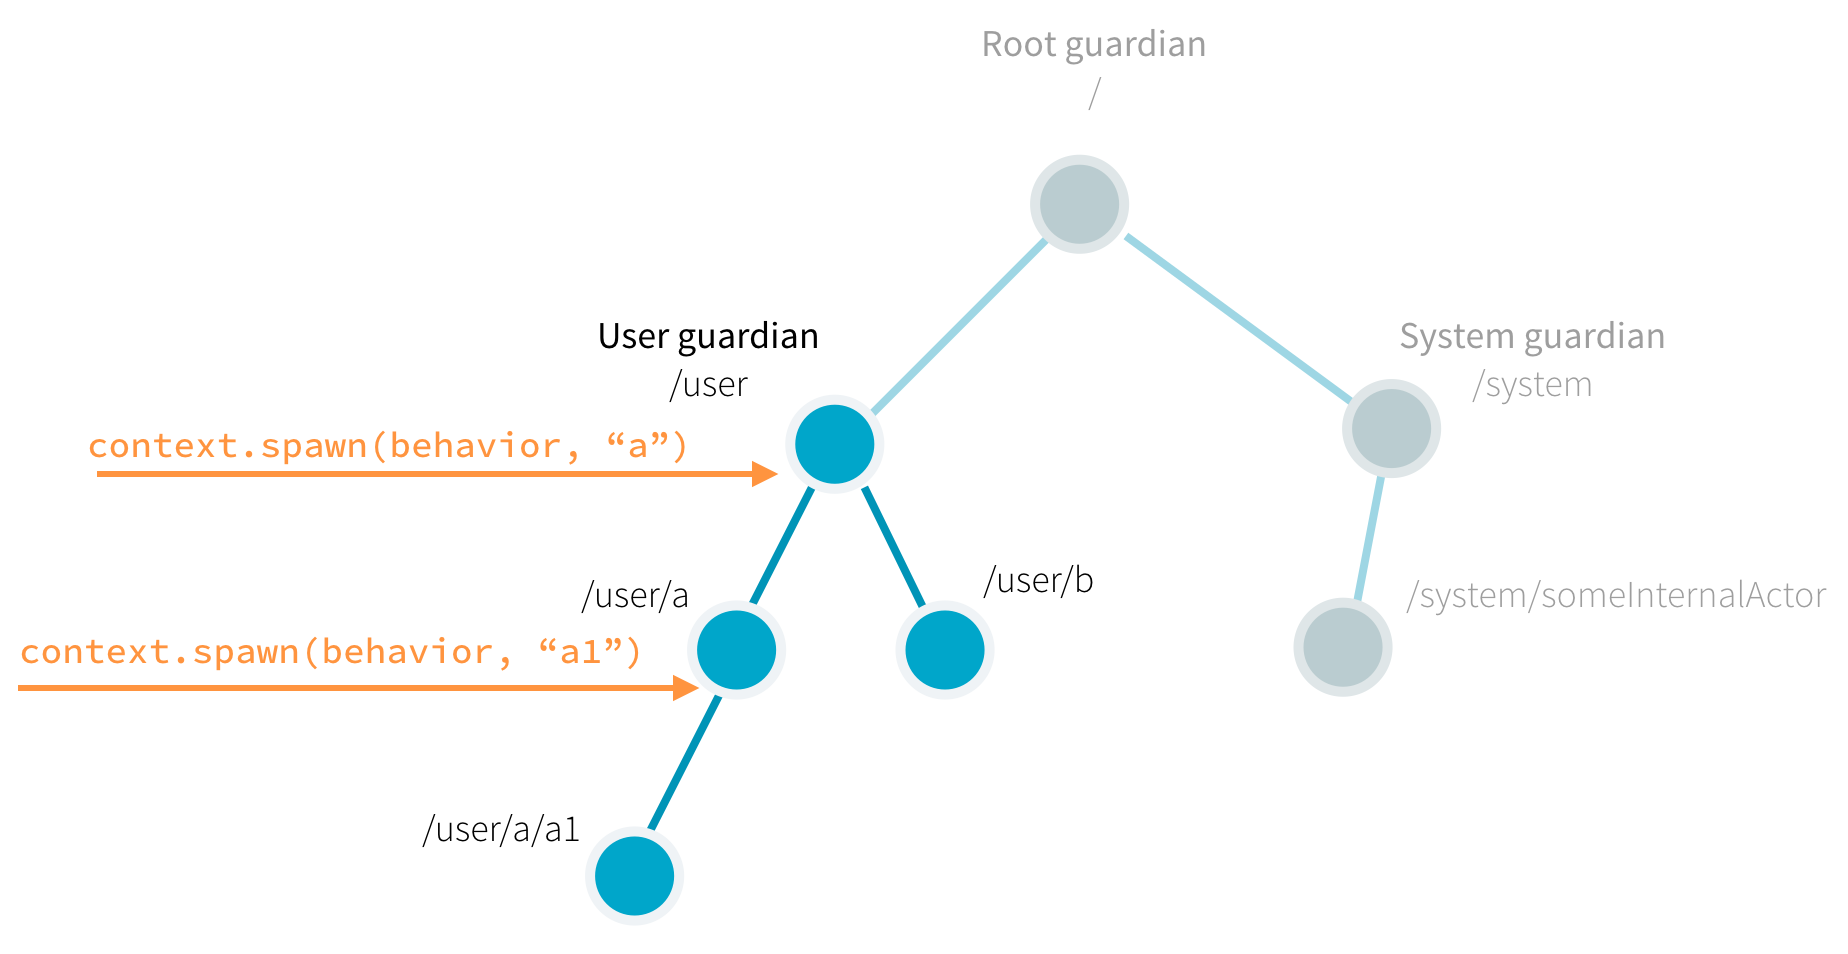
\includegraphics[width = 0.6\textwidth]{actor_top_tree.png}
  \caption[Gerarichia degli Attori]{Albero delle gerarichia degli Attori}
\end{figure}

Le strategie di gestione dei fallimenti possono essere personalizzate per rispondere alle specifiche esigenze del sistema o selezionate tra quelle fornite dal toolkit:
\begin{itemize}
  \item \textbf{Restart}: l'attore viene ricreato attraverso il proprio factory method, riprendendo immediatamente l'attività. Gli altri attori continuano a referenziare l'attore utilizzando un riferimento logico costante esternamente.
  \item \textbf{Resume}: l'attore prosegue con l'elaborazione dei messaggi, ignorando il fallimento.
  \item \textbf{Stop}: l'attore viene terminato, impedendogli di continuare a elaborare messaggi.
  \item \textbf{Escalate}: il supervisore trasferisce la problematica al proprio supervisore.
\end{itemize}
Adottare l'approccio \textit{let it crash} offre notevoli vantaggi.
Consente al supervisore di gestire gli errori sollevati dagli attori supervisionati senza compromettere le relazioni con gli altri attori.
Questi ultimi, quando possibile, continuano a scambiare messaggi con una nuova istanza dell'attore fallito piuttosto che con lo stesso attore ripristinato, assicurando un recupero senza soluzione di continuità. 

Per illustrare concretamente questa metodologia, consideriamo il seguente frammento di codice.
Qui definiamo un attore supervisore, \textit{HelloWorldSupervisorActor}, che stabilisce una strategia comune per gli attori figli supervisionati, come ad esempio "\textit{HelloWorldActor}."
Questa strategia è selezionata in base all'eccezione lanciata dal figlio, evidenziando la flessibilità e l'efficacia nella gestione delle situazioni di errore all'interno del contesto attoriale.
Questo approccio riflette la sofisticata architettura di Akka, che permette una gestione dinamica e scalabile degli errori in scenari reali e complessi.

\lstinputlisting[language=Scala, float=ht]{code/Messages.java} 

\subsubsection[Location transparency]{Location transparency}
Il meccanismo di localizzazione degli attori in Akka si basa su un servizio di naming distribuito, un pilastro cruciale per l'architettura di sistemi attoriali che mirano alla scalabilità e alla distribuzione.
Ogni singolo attore è distintamente identificato all'interno di uno spazio utente condiviso attraverso un riferimento logico noto come \textit{actorRef}, il quale è successivamente mappato da un percorso che segue la struttura gerarchica degli attori fino a raggiungere la radice del sistema. \\
Parallelamente, è presente un riferimento fisico noto al sistema, denominato \textit{actorPath}, che consente il riconoscimento univoco di un attore.
Questo riferimento è rappresentato da una stringa strutturata nel seguente formato:
\begin{lstlisting}
  protocol://actorSystem@hostname:port/actorPath`  
\end{lstlisting}
Per esempio, consideriamo l'\textit{actorPath}:
\begin{lstlisting}
  akka.tcp://mySystem@myHost:9001/user/myActor`
\end{lstlisting}
che identifica l'attore denominato \textit{myActor} nel contesto del sistema Akka chiamato \textit{mySystem}.
Quest'ultimo è in esecuzione sulla macchina denominata \textit{myHost}, ascoltando sulla porta 9001 attraverso il protocollo \textit{tcp}. 

Quando il programmatore necessita di localizzare un attore, utilizza esclusivamente il riferimento logico, trascurando la necessità di conoscere la reale locazione dell'attore, che potrebbe essere sia locale che remota.
La responsabilità di risolvere il riferimento logico in un riferimento fisico è affidata al sistema, garantendo così una gestione trasparente e efficiente della distribuzione degli attori. \\
Il riferimento logico, oltre a essere utilizzato per operazioni di lookup degli attori da parte del sistema, viene implicitamente incorporato come mittente nei messaggi, semplificando le interazioni tra attori.
Inoltre, attraverso l'utilizzo del componente \textit{ActorSelection}, è possibile recuperare il riferimento logico insieme ad altri riferimenti.
Questo componente consente l'applicazione di \textit{wildcard}, facilitando la localizzazione su larga scala di più attori.
L'architettura di naming distribuito implementata in Akka costituisce un elemento chiave che offre un alto livello di astrazione.
Ciò consente ai programmatori di concentrarsi sulla logica applicativa, mentre il sistema gestisce in modo efficiente e trasparente la complessità della distribuzione degli attori.
Tale approccio fornisce una flessibilità e una scalabilità superiori nell'implementazione di sistemi complessi e distribuiti.

\begin{figure}[H]
  \centering
  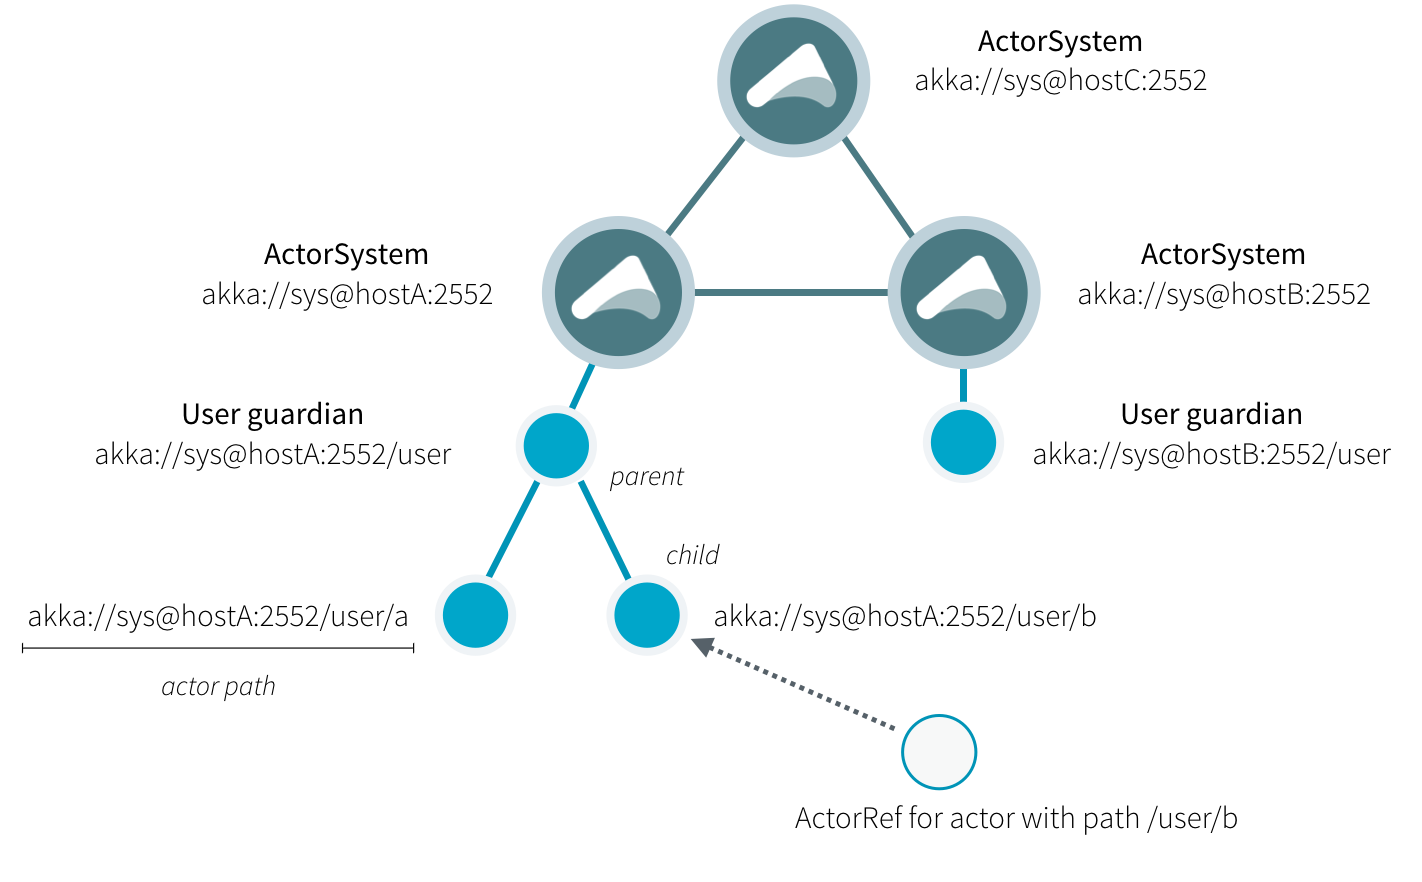
\includegraphics[width = 0.6\textwidth]{actor-paths-overview.png}
  \caption[Percorso degli attori]{Panoramica del percorso degli attori}
\end{figure}

\subsubsection[Routing, scalabilità e clustering]{Routing, scalabilità e clustering}
Per assicurare la sostenibilità delle prestazioni di fronte alla crescente domanda, è essenziale adottare strategie di scalabilità nel sistema di attori.
Questo può avvenire attraverso gli approcci tradizionali di \textit{scale up} e \textit{scale out}. \\
Nel caso dello \textit{scale up}, si potenzia il sistema verticalmente mediante l'aggiunta di attori locali al nodo esistente.
In alternativa, con lo "\textit{scale out}", si introduce un nuovo nodo remoto nel cluster di sistema, includendo nuovi attori.

La gestione efficiente delle richieste è ottimizzata attraverso l'impiego di attori specializzati noti come \textit{Router}.
Questi attori indirizzano le richieste attraverso azioni definite per i Routee, creando e gestendo diverse istanze dello stesso tipo di attore mediante un \textit{actor-pool}.
Un'ulteriore ragione per l'adozione del routing potrebbe derivare dalla necessità di selezionare il \textit{Routee} in base al messaggio trasmesso o allo stato interno del router.
Akka offre una gamma di strategie di routing predefinite:
\begin{itemize}
  \item \textit{Round Robin}: selezione ciclica dei Routee senza priorità.
  \item \textit{Random}: selezione casuale dei Routee.
  \item \textit{Smallest Mailbox}: instradamento basato sulla mail-box con meno messaggi in coda.
  \item \textit{Balancing Pool}: condivisione della stessa mail-box tra tutti i Routee, con il router che distribuisce i messaggi ai Routee liberi.
  \item \textit{Broadcast}: distribuzione del medesimo messaggio a tutti i Routee.
  \item \textit{Scatter-Gather First Completed}: simile al broadcast, ma con il router che attende la prima risposta tra i Routee entro un intervallo di tempo specifico.
  \item \textit{Tail Chopping}: il router invia il messaggio a un Routee selezionato casualmente, applicando questa logica a intervalli regolari fino alla ricezione della prima risposta.
  \item \textit{Consistent Hashing}: instradamento basato sull'hashing del messaggio.
\end{itemize}
Ricordando la flessibilità di Akka nell'implementazione di applicazioni distribuite, ciò è realizzato attraverso la definizione di tecniche di clustering.
Questo consente l'espansione orizzontale mediante l'aggiunta di nodi al cluster, in cui ciascun nodo appartiene a una rete peer-to-peer e mantiene la sincronizzazione attraverso il protocollo di gossip con gli altri nodi.
Ciò agevola il lookup degli attori in modo indipendente dalla loro localizzazione fisica, promuovendo la \textit{location transparency}, e permette il rilevamento delle cadute di altri nodi.
L'obiettivo primario del cluster è garantire la fault tolerance in caso di fallimento di un nodo e il load balancing per distribuire in modo efficiente i messaggi ai vari nodi.
Inoltre, un \textit{actor system} può essere suddiviso in partizioni dislocate su nodi diversi per soddisfare esigenze prestazionali specifiche.

\subsubsection[Ecosistema]{Ecosistema AKKA}
Akka, analogamente a numerosi framework nel campo del Big Data, dispone di un proprio ecosistema ricco di librerie progettate per soddisfare le esigenze tradizionali che possono emergere nello sviluppo di soluzioni enterprise.
Questo insieme di moduli amplia le capacità di Akka e ne favorisce l'integrazione in contesti complessi.

\begin{itemize}
  \item Il concetto chiave di Akka è rappresentato dagli \textit{Actors}, che costituiscono il fondamento del modello ad attori.
  Questo paradigma offre una soluzione elegante per affrontare le sfide della programmazione concorrente, consentendo la gestione efficiente delle comunicazioni e degli stati all'interno di un sistema distribuito.
  \item Il modulo \textit{Streams} amplia ulteriormente la capacità di Akka di gestire flussi di dati in modo asincrono e non bloccante.
  Questa caratteristica è fondamentale in scenari in cui è necessario elaborare continuamente un elevato volume di informazioni, come nel caso di applicazioni che trattano dati in tempo reale o in ambienti in cui la latenza è critica.
  \item L'implementazione di un server HTTP leggero, fornita dal modulo \textit{HTTP}, aggiunge un elemento di flessibilità e efficienza alle applicazioni Akka, specialmente in contesti in cui è richiesto un trattamento ottimizzato delle richieste web.
  Questo si traduce in una maggiore capacità di gestire carichi di lavoro intensi e rispondere alle richieste degli utenti in modo rapido ed efficiente.
  \item Il modulo \textit{Cluster} introduce concetti cruciali come resilienza e scalabilità attraverso l'adozione di tecniche di clustering.
  Questo è particolarmente significativo in scenari in cui la disponibilità continua del servizio è essenziale, garantendo che il sistema sia in grado di adattarsi dinamicamente alle variazioni del carico di lavoro e di gestire efficacemente eventuali guasti hardware.
  \item La distribuzione programmabile degli attori tramite il modulo \textit{Sharding} fornisce un meccanismo potente per ottimizzare l'allocazione delle risorse in un ambiente distribuito.
  Ciò consente di massimizzare l'utilizzo delle risorse e migliorare l'efficienza complessiva del sistema.
  \item Il modulo \textit{Distributed Data} contribuisce alla coerenza e alla sincronizzazione dei dati tra i nodi, fornendo un key-value store distribuito.
  Questo è essenziale per garantire che i dati siano sempre aggiornati e consistenti in un ambiente in cui la distribuzione dei dati è una sfida chiave.
  \item La persistenza dello stato, implementata attraverso il modulo \textit{Persistence} utilizzando il pattern event-sourcing, offre una soluzione robusta per gestire la memorizzazione e il recupero degli stati del sistema.
  Questo è particolarmente rilevante in applicazioni in cui la tracciabilità degli eventi passati è essenziale per comprendere lo stato attuale del sistema.
  \item \textit{Alpakka} si distingue per il suo focus sul reactive streaming e la sua libreria dedicata all'integrazione con Apache Kafka e server applicativi di tipo gRPC.
  Ciò amplia ulteriormente le capacità di Akka nel trattare flussi di dati reattivi e nella connessione con altri sistemi distribuiti, offrendo un'integrazione senza soluzione di continuità con tecnologie ampiamente utilizzate nell'ecosistema Big Data.
  \item Infine, il modulo "\textit{Management}" estende l'utilizzo di Akka su sistemi Cloud, offrendo un'implementazione semplificata e ottimizzata per ambienti basati su servizi cloud. 
  Ciò riflette l'impegno di Akka nel rimanere al passo con le tendenze emergenti nella distribuzione delle applicazioni e nell'adozione di architetture cloud-native.
\end{itemize}
Inoltre, l'azienda Lightbend ha sviluppato il framework \textit{Play} come complemento a Akka, offrendo un ambiente di sviluppo completo per la creazione di soluzioni web in Scala e Java.
L'integrazione di Akka all'interno del motore di Play sottolinea la coerenza e la sinergia tra questi framework, offrendo agli sviluppatori una piattaforma completa e potente per affrontare sfide complesse nello sviluppo di applicazioni web avanzate e scalabili.

\subsubsection[Pattern]{Pattern e Anti-Pattern}
L'implementazione del modello ad attori introduce una fase iniziale di adozione caratterizzata da un elevato tasso di errore nell'assimilazione dei principi fondamentali.
Pertanto, risulta prezioso delineare in maniera sintetica i pattern e, altrettanto significativo, gli anti-pattern da considerare attentamente durante la fase di progettazione di soluzioni basate sul modello ad attori, implementate tramite Akka.

Tra i pattern riconosciuti, è opportuno evidenziare:
\begin{itemize}
  \item \textbf{Decomposizione del Lavoro}: un principio cardine consiste nella distribuzione del lavoro tra più attori, seguendo un paradigma di separazione delle responsabilità. Evitando un centralismo operativo, si favorisce una maggiore flessibilità e adattabilità del sistema.
  \item \textbf{Immutabilità dei Messaggi}: i messaggi devono essere rappresentati esclusivamente da oggetti immutabili, assicurando coerenza e prevenendo problemi di concorrenza derivanti da modifiche simultanee.
  \item \textbf{Gerarchia di Attori}: la creazione di attori in una gerarchia adeguata favorisce l'implementazione di strategie di supervisione efficaci, contribuendo alla gestione di eventuali errori in modo strutturato e robusto.
  \item \textbf{Incapsulamento di Stato e Comportamenti}: sia lo stato di ciascun attore sia i relativi comportamenti devono essere incapsulati e non accessibili dall'esterno, promuovendo una corretta gestione degli oggetti e minimizzando l'interferenza esterna.
  \item \textbf{Messaggistica Asincrona}: l'invio dei messaggi deve avvenire in modo asincrono e non bloccante, adottando un approccio fire-and-forget che incrementa l'efficienza e la reattività del sistema.
\end{itemize}

D'altra parte, tra gli anti-pattern da evitare si possono individuare:
\begin{itemize}
  \item \textbf{Stato Interno Pubblico e Mutabile}: evitare la definizione di uno stato interno pubblico e mutabile, che sarebbe accessibile e modificabile dall'esterno, compromettendo la stabilità e la coerenza del sistema.
  \item \textbf{Gerarchia "\textit{Piatta}" di Attori}: la definizione di una gerarchia "piatta" degli attori dovrebbe essere evitata, in quanto una struttura gerarchica più articolata facilita la gestione degli attori e delle loro interazioni.
  \item \textbf{Eccessiva Complessità nell'Esecuzione}: limitare l'esecuzione di numerosi actor system sullo stesso nodo, o l'esecuzione di un eccessivo numero di attori all'interno di uno stesso actor system. In alternativa, distribuire gli actor system su nodi distinti e distribuiti, evitando sovraccarichi e migliorando la scalabilità.
  \item \textbf{Messaggistica Sincrona e Bloccante}: l'invio sincrono e bloccante di messaggi, soprattutto nel contesto request-response, va evitato per preservare la fluidità e la tempestività del sistema.
  \item \textbf{Definizione di Comportamenti Sensibili alle Race Condition}: evitare la definizione di comportamenti degli attori influenzati dal fenomeno delle race condition, in cui il risultato finale è dipendente dall'ordine di elaborazione dei singoli task in un contesto concorrente.
\end{itemize}

Comprensione accurata e attenta applicazione di tali pattern e anti-pattern è cruciale per garantire la corretta implementazione di soluzioni basate sul modello ad attori, consentendo la realizzazione di sistemi robusti, scalabili e adattabili alle sfide dell'ambiente distribuito.

    \chapter[Pipeline predittiva]{Progettazione e implementazione di un software predittivo}
    La concezione di software predittivo sorge dall'impellente necessità di elaborare vasti volumi di dati entro tempi \textit{ragionevoli}, avvicinandosi al concetto di near real-time.
In questo contesto, il periodo di attesa per l'ottenimento di risposte, generalmente nell'ordine di secondi, si colloca certamente al di sopra dei sistemi real-time, ma notevolmente al di sotto dei sistemi batch.
La realizzazione di questo software implica la definizione e la sincronizzazione di tutti i suoi componenti mediante l'adozione del modello ad attori.
Tale approccio coinvolge in modo sinergico framework esterni specializzati nel calcolo parallelo distribuito, nell'orchestrazione dei messaggi e nella gestione dello storage distribuito. \\
L'architettura del software, in contrasto con i tradizionali sistemi batch, è improntata a un'efficienza temporale significativa, consentendo un'analisi e un apprendimento continuo su grandi quantità di dati.
La synchronicità tra i componenti, ottenuta attraverso il modello ad attori, offre un livello di parallelismo e distribuzione delle responsabilità fondamentale per fronteggiare le sfide della gestione di grandi flussi informativi. \\
La collaborazione con framework esterni specializzati nell'esecuzione di calcoli paralleli distribuiti consente di sfruttare al massimo la potenza computazionale disponibile, accelerando i processi di analisi e apprendimento del software.
L'integrazione di meccanismi di brokering dei messaggi facilita una comunicazione fluida e efficiente tra i diversi componenti, garantendo coerenza e tempestività nell'elaborazione delle informazioni. \\
Inoltre, il software si avvale di soluzioni di storage distribuito, contribuendo così alla gestione ottimizzata dei dati.
Questi sistemi di storage distribuito consentono l'accesso rapido e affidabile ai dati necessari per l'analisi, garantendo al contempo la resilienza e la ridondanza necessarie per affrontare eventuali guasti o perdite di dati.

\section[Descrizione generale]{Una descrizione generale}
In questo contesto, il software si configura come un sostegno fondamentale per l'implementazione di modelli di Machine Learning e Advanced Analytics, fornendo un layer di astrazione composto da un insieme di classi astratte che generalizzano comportamenti e operazioni.
Questo strato di astrazione facilita l'interazione con vari framework di Big Data impiegati per la realizzazione di modelli di apprendimento automatico.
Il software segue il flusso dei dati dalla fase di generazione iniziale attraverso l'elaborazione fino al salvataggio, delineando una struttura applicativa ben definita. \\
All'interno del software, emergono tre macro layer applicativi di riferimento:
\begin{itemize}
    \item Il primo strato si occupa della gestione e trasmissione dei dati di input.
    \item Il secondo gestisce il routing delle richieste.
    \item Il terzo costituisce il nucleo di analisi, caratterizzato dalle attività di apprendimento automatico e analisi avanzata.
\end{itemize}

Un elemento distintivo del software è l'approccio di disaccoppiamento del layer di analisi dal resto del sistema.
Questo disaccoppiamento si manifesta attraverso due job indipendenti per la creazione e l'addestramento di modelli di Machine Learning e per l'analisi avanzata dei dati.
Tali job vengono eseguiti periodicamente in modo autonomo rispetto alle altre componenti del sistema.
Alla conclusione di ogni iterazione, i risultati generati sono immediatamente trasmessi alle componenti interessate, pronte per l'utilizzo in sostituzione di quelli precedentemente memorizzati nei rispettivi buffer di memoria.

La componente dedicata al Machine Learning assume il compito di generare modelli di classificazione, basandosi su dati storici presenti nel file system distribuito e su dati in tempo reale elaborati dalla piattaforma.
La flessibilità del software come sistema adattivo è evidente nella sua capacità di arricchire continuamente il training set con ogni messaggio prodotto e analizzato.
Al termine di ogni generazione, viene selezionato, tra gli algoritmi classificazione utilizzati, quello che meglio si adatta e dimostra maggiore accuratezza rispetto ai dati disponibili nello stato attuale del sistema.
La dinamicità di questo processo contribuisce a mantenere la pipeline di intelligenza artificiale adattata e ottimizzata in risposta alle variazioni nei dati e alle esigenze dell'applicazione.

\section[Architettura]{L'architettura del software}
Il software predittivo è concepito e sviluppato implementando il modello ad attori, in cui ogni componente applicativa è realizzato seguendo il paradigma dell'attore. \\
La decisione di utilizzare il linguaggio di programmazione Scala si basa sulla sua intrinseca adattabilità a contesti in cui la scalabilità è un requisito cruciale.
Scala offre un equilibrio unico tra conciseness e potenza, consentendo lo sviluppo di codice efficiente e manutenibile.
La sua interoperabilità con Java fornisce inoltre un ampio accesso a librerie e framework consolidati nel mondo dello sviluppo software. \\
Il software predittivo, attraverso la sua implementazione basata su attori, promuove la separazione delle responsabilità e la modularità dei componenti.
Ogni attore rappresenta un'unità autonoma di esecuzione, contribuendo a una gestione più agevole dei processi distribuiti.
La comunicazione tra attori avviene in modo asincrono, migliorando la reattività e la flessibilità del sistema nell'adattarsi alle varie esigenze di previsione. \\
La scalabilità, quale requisito fondamentale del software predittivo, diventa una caratteristica distintiva grazie alla sua implementazione basata su attori e al linguaggio Scala.
La capacità di gestire carichi di lavoro crescenti o variabili è intrinseca nel modello ad attori, che permette di aggiungere o rimuovere attori in risposta alla dinamica del sistema.

\subsection[Componenti]{Le componenti del software}
La concezione del software predittivo si fonda su una pipeline strutturata, che incorpora diverse componenti essenziali per garantire un flusso efficiente e reattivo nel processo predittivo:

\subsubsection[Producer]{Producer} 
Il Prodcuer è un attore specificamente designato a monitorare in maniera continua il dataset raw generato dai dispositivi o sistemi di origine.
Questo dataset costituisce l'input cruciale per l'intera pipeline predittiva, alimentando il processo di analisi e previsione.
Il ruolo del Producer è di vitale importanza, poiché, in modo costante, analizza il dataset raw alla ricerca di variazioni nei file in esso contenuti. \\
Ogni volta che si verifica una modifica, il Producer riceve una notifica di cambiamento e prontamente reagisce accodando un nuovo messaggio di input verso il message broker.
Questo meccanismo di notifica e risposta assicura che il software predittivo sia sempre allineato con l'evoluzione dinamica del dataset raw, consentendo un processo di predizione tempestivo e accurato. \\
L'integrazione del Producer nella pipeline del software predittivo sottolinea la necessità di una sorveglianza continua e di un'adeguata gestione degli input.
Questo attore svolge un ruolo cruciale nell'assicurare la coerenza e l'aggiornamento costante dei dati utilizzati per le analisi predittive.
La sua capacità di rilevare rapidamente le variazioni e di reagire prontamente garantisce che il flusso di input sia sempre allineato con le dinamiche in tempo reale dell'ambiente di rilevamento.

\subsubsection[Consumer]{Consumer}
Il Consumer all'interno della struttura operativa è l'incaricato di gestire il processo di estrazione e analisi dei nuovi messaggi di input pervenuti attraverso il message broker.
La sua versatilità si manifesta nella capacità di adattarsi a diverse tipologie di messaggi, ognuna specifica per il contesto di studio.
La sua funzione principale consiste nell'interpretare il tipo di messaggio ricevuto e intraprendere azioni mirate in base alla sua natura. \\
Una volta che il Consumer ha estratto un nuovo messaggio di input dal message broker, si impegna in un'analisi approfondita.
La sua capacità di discernere la tipologia di messaggio diventa cruciale, poiché il percorso successivo è determinato dalla natura specifica del messaggio.
In base al contesto di studio, il Consumer è programmato per instradare il messaggio verso il predittore nel caso di richieste di previsione.
Se invece il messaggio è una richiesta di recupero di dati statistici, il Consumer lo instraderà verso il feeder.
Nel caso in cui il messaggio rappresenti un output raw, il Consumer provvederà a salvare il dato nel file system distribuito, arricchendo ulteriormente il training set del sistema. \\
La flessibilità del Consumer nell'adattarsi alle diverse tipologie di input e nell'effettuare le scelte di instradamento in base al contesto dimostra la sua centralità all'interno del flusso operativo del sistema.
La sua azione di istruzione dei messaggi contribuisce in modo significativo alla definizione del percorso e alla destinazione finale dei dati, fornendo così un'organizzazione strutturata e coerente alle informazioni elaborate.

\subsubsection[Trainer]{Trainer}
Il Trainer si configura come l'attore principale incaricato della creazione e dell'addestramento dei modelli di Machine Learning.
La sua esecuzione avviene in maniera periodica, intervallata da specifici intervalli temporali, durante i quali recupera sia i dati storici archiviati, sia quelli raccolti dalla piattaforma nel corso delle sue attività operative.
La sua azione di recupero dati si estende sia al training set rigenerato ad ogni iterazione, che costituisce la base essenziale per il processo di apprendimento automatico, sia ai nuovi dati provenienti dai test set. \\
La fase di addestramento è un momento critico per il Trainer, che sfrutta i dati acquisiti per generare diversi modelli di Machine Learning.
Questi modelli sono poi applicati a nuovi test set per valutare le loro performance.
La selezione del modello ottimale avviene in base a specifiche metriche distinte, delineate in funzione delle esigenze del contesto applicativo.
Nel caso di modelli di regressione, ad esempio, l'efficacia potrebbe essere valutata mediante metriche come l'errore quadratico medio, mentre per i modelli di classificazione potrebbero essere considerati indicatori come precisione e recall. \\
La fondamentale caratteristica del Trainer risiede nella sua capacità di adattarsi e migliorarsi continuamente.
La rigenerazione del training set ad ogni iterazione consente al Trainer di integrare nuovi dati e di affinare progressivamente i modelli di Machine Learning, garantendo un apprendimento continuo e dinamico.
La diversificazione dei modelli generati e la selezione del migliore costituiscono un passo cruciale nell'evoluzione del sistema, permettendo di mantenere elevata l'accuratezza delle previsioni nel tempo. \\
La fase conclusiva dell'elaborazione del Trainer prevede la trasmissione del modello ottimale al rispettivo predittore.
Questo collegamento diretto garantisce che il modello addestrato sia prontamente utilizzato per effettuare previsioni nel contesto operativo del sistema predittivo, contribuendo a mantenere il sistema allineato con l'andamento dinamico dei dati. \\

\subsubsection[Analyzer]{Analyzer}
L'Analyzer si configura come l'attore preposto alla generazione di dati statistici relativi al dataset storico e alle informazioni acquisite in tempo reale dalla piattaforma.
Il suo processo operativo è caratterizzato da una periodica esecuzione, intervallata da specifici intervalli temporali, durante i quali esegue un'analisi approfondita dei dati a disposizione.
Una volta completata l'analisi, l'Analyzer trasmette i risultati ottenuti al feeder, contribuendo così alla raccolta di informazioni dettagliate e significative per il sistema nel suo complesso. \\
La responsabilità chiave dell'Analyzer consiste nella generazione di dati statistici accurati e informativi.
Esso svolge questa funzione sia sul dataset storico, costituito dai dati archiviati nel tempo, sia sui dati acquisiti in tempo reale, provenienti dalla continua attività della piattaforma.
Questo approccio integrato garantisce un'analisi completa e dinamica, incorporando sia le tendenze passate che gli sviluppi immediati, offrendo così una visione completa dell'ambiente operativo. \\
L'esecuzione periodica dell'Analyzer rafforza la sua capacità di mantenere aggiornati i dati statistici, consentendo una comprensione sempre attuale e precisa delle dinamiche di sistema.
Ogni intervallo di esecuzione si traduce in un nuovo set di dati statistici, permettendo al sistema di adattarsi in tempo reale alle variazioni nell'ambiente e di rispondere con prontezza alle nuove sfide o opportunità che possono emergere. \\
L'invio regolare dei risultati all'interno del Feeder contribuisce alla coerenza e all'integrità del flusso informativo all'interno del sistema predittivo.

\subsubsection[Predictor]{Predictor}
Il Predictor assume il ruolo fondamentale di ricevere richieste di predizione e di soddisfarle attraverso l'impiego di modelli generati precedentemente dal Trainer.
La sua operatività si caratterizza per la gestione accurata delle richieste di previsione provenienti da altre componenti della pipeline, fungendo da ponte essenziale tra la fase di addestramento dei modelli e l'applicazione pratica delle previsioni nel contesto operativo. \\
La funzione primaria del Predictor è di mantenere costantemente in memoria una copia del modello attualmente utilizzato.
Questa pratica garantisce una risposta tempestiva e senza ritardi alle richieste di predizione, evitando la necessità di ricaricare il modello ad ogni richiesta.
Parallelamente, il Predictor si impegna a sostituire la copia in memoria con un nuovo modello appena ricevuto dal Trainer.
Questo processo di aggiornamento regolare consente al sistema di adattarsi dinamicamente alle modifiche nei dati e nell'ambiente operativo, migliorando costantemente la precisione delle previsioni. \\
La memoria persistente del modello nel Predictor riflette la sua capacità di mantenere una conoscenza consolidata dei modelli di Machine Learning, facilitando un accesso rapido e efficiente ai dati di apprendimento.
Questo approccio consente di evitare la necessità di ricaricare il modello ad ogni richiesta di predizione, riducendo il tempo di risposta e migliorando l'efficienza complessiva del sistema predittivo. \\
La sincronizzazione tra il Predictor e il Trainer è un elemento chiave nel garantire la coerenza e l'affidabilità delle previsioni.
La prontezza nel sostituire il modello in uso con la versione più recente fornita dal Trainer consente al sistema di adottare immediatamente nuovi pattern e tendenze emerse dai dati più recenti, contribuendo a mantenere l'efficacia delle previsioni nel tempo.

\subsubsection[Feeder]{Feeder}
Il Feeder assume il ruolo chiave di fornire dati statistici in risposta a richieste specifiche.
Parallelamente al Predictor, il Feeder si occupa di gestire il flusso di dati statistici generati dall'Analyzer, svolgendo un ruolo essenziale nella distribuzione coerente e tempestiva delle informazioni attraverso il sistema.
La sua funzione principale è quella di mantenere in memoria una copia del dataset statistico ottenuto dall'Analyzer, una riserva di dati chiave che viene sostituita con la versione più recente ogni volta che è disponibile. \\
La gestione oculata dei dati statistici da parte del Feeder riveste importanza cruciale nel garantire che le richieste specifiche provenienti da altri attori della pipeline siano soddisfatte in modo efficiente.
Il Feeder funge da intermediario affidabile, consentendo agli attori successivi, come il Predictor, di accedere rapidamente a dati statistici rilevanti senza dover eseguire nuovamente analisi complesse sull'intero dataset. \\
Parallelamente al processo di sostituzione del dataset statistico, il Feeder si impegna anche a rispondere prontamente alle richieste specifiche provenienti dal resto del sistema.
La sua capacità di fornire dati statistici dettagliati, senza la necessità di ricorrere a analisi complesse ad ogni richiesta, migliora significativamente l'efficienza del sistema nel compiere previsioni e decisioni informate. \\
La sincronizzazione tra il Feeder e il Predictor, entrambi dotati di una copia aggiornata del dataset statistico, consente una coerenza nell'accesso ai dati e contribuisce a mantenere l'accuratezza delle previsioni nel tempo.
La prontezza nel sostituire il dataset memorizzato con la versione più recente assicura che il sistema operi costantemente con informazioni aggiornate, migliorando la sua capacità di adattamento alle variazioni nell'ambiente operativo.

\section[Pipeline]{La pipeline}
Nella fase di \textit{bootstrap}, si procede alla creazione e all'avvio degli attori fondamentali, quali il Producer, il Consumer, il Trainer e l'Analyzer, stabilendo così le basi operative del sistema predittivo.

Durante l'avvio, il Consumer, tramite \textit{ActorRef}, acquisisce il riferimento logico al Predictor e al Feeder, istituendo una connessione essenziale per le future richieste di predizione.
L'operatività del Trainer si svolge a intervalli regolari, e il suo compito principale consiste nella costruzione dei modelli di Machine Learning.
In questo processo, il Trainer delega ai componenti specifici del caso di studio tutto ciò che non può essere generalizzato, concentrandosi principalmente sulla fase di \textit{feature engineering}.
Attraverso l'accesso a HDFS, il Trainer recupera sia i dati storici sia quelli acquisiti in tempo reale, dando vita a dataset di training e di test in modo casuale.
La costruzione del modello avviene utilizzando i dati di training, mentre la fase di verifica viene eseguita sui dati di test.

L'approccio periodico del Trainer nel generare modelli riflette la sua capacità di adattarsi e migliorarsi continuamente.
La regolarità degli intervalli di esecuzione permette al Trainer di integrare nuovi dati in modo sistematico e di affinare costantemente i modelli, assicurando un apprendimento dinamico e aggiornato rispetto alle evoluzioni dell'ambiente. \\
L'interazione del Consumer con il Predictor e il Feeder all'inizio del processo sottolinea la sinergia necessaria per il flusso operativo del sistema.
Questa connessione precoce tra attori assicura che le richieste future siano gestite in modo fluido e tempestivo, garantendo una comunicazione efficiente tra le diverse componenti della pipeline. 

Alla conclusione della fase di addestramento del Trainer, si avvia una sequenza di operazioni essenziali eseguite dall'Analyzer, elemento fondamentale nella pipeline del sistema predittivo.
Inizialmente, l'Analyzer si impegna nel calcolare una serie di metriche specifiche, che variano in base alla tipologia di algoritmo adottato, sia esso di tipo regressione o classificazione.
Questo processo di valutazione mira a determinare l'accuratezza dei modelli generati, fornendo una base critica per la selezione del modello più preciso.
Una volta identificato il modello ottimale, l'Analyzer procede a trasmetterlo al Predictor per l'utilizzo pratico nelle future richieste di predizione. \\
Parallelamente, l'Analyzer svolge un ruolo attivo nella conservazione e nell'organizzazione dei risultati ottenuti.
Salvando su file system i dettagli delle misure effettuate, l'Analyzer crea un registro dettagliato delle prestazioni dei modelli, offrendo una risorsa di riferimento preziosa per valutazioni future e analisi retrospettive.
In aggiunta, genera strutture dati cruciali per l'analisi avanzata: una matrice di correlazione per i modelli di regressione e una matrice di confusione per quelli di classificazione.
Queste strutture forniscono un'ulteriore profondità di comprensione sul comportamento dei modelli, permettendo una visione dettagliata delle relazioni tra le variabili o delle prestazioni nel caso di classificazione. \\
L'esecuzione periodica dell'Analyzer, intervallata a scadenze regolari, costituisce un aspetto significativo della sua operatività. \\
Durante ogni esecuzione, l'Analyzer calcola una serie di statistiche specifiche definite all'interno delle componenti specializzate per ciascun caso di studio.
Questo approccio mirato consente all'Analyzer di adattarsi alle esigenze specifiche di ogni contesto applicativo, contribuendo a garantire che le statistiche rilevanti vengano catturate e analizzate con precisione. \\
L'efficace recupero di dati da HDFS da parte dell'Analyzer, unito alla sua capacità di notificare tempestivamente i risultati al Feeder, sottolinea l'integrazione sinergica di questa componente nella pipeline complessiva del sistema predittivo.
La trasmissione pronta delle informazioni al Feeder alimenta la coerenza e l'efficienza del flusso operativo, consentendo al sistema di rimanere agilmente rispondere alle dinamiche mutevoli dell'ambiente. 

Il Producer viene attivato in risposta a qualsiasi variazione rilevata nel dataset di input da esso monitorato.
A ogni modifica del dataset, esso prende l'iniziativa di trasmettere i nuovi dati al topic Kafka.
Questo processo garantisce una gestione dinamica e reattiva del flusso di dati, garantendo che qualsiasi cambiamento nell'input venga prontamente catturato e trasmesso agli altri componenti della pipeline. \\
Il Consumer, a sua volta, ha il compito di estrarre i dati appena trasmessi dal topic Kafka.
La sua operatività è basata sulla capacità di analizzare il tipo di input ricevuto e di prendere decisioni immediate in merito alla successiva instradazione del messaggio.
In base alle caratteristiche dell'input, il Consumer decide se indirizzare il messaggio al componente Predictor, per la predizione utilizzando il modello più recente generato dal Trainer, o se inviarlo al Feeder, per ottenere il dataset statistico più recente dal Analyzer. \\
Il Predictor utilizza il modello più recente generato dal Trainer per eseguire la previsione.
La risposta predittiva viene poi restituita al Consumer, completando così il ciclo operativo.

Questo approccio assicura che il sistema si avvalga costantemente delle informazioni più aggiornate per effettuare previsioni accurate e tempestive. \\
Dall'altro lato, il Feeder svolge un ruolo complementare fornendo al Consumer il dataset statistico più recente generato dall'Analyzer.
Questa sinergia tra il componente che effettua le previsioni e quello che fornisce dati statistici attuali consente al sistema di operare in modo coerente e integrato. \\
Un passaggio fondamentale nel processo operativo è la memorizzazione su file system locale dei risultati ottenuti, compito affidato al Consumer.
Questa pratica contribuisce a mantenere un registro storico delle operazioni, facilitando future analisi, monitoraggi e audit delle attività svolte dal sistema predittivo.

\section[Scalabilità]{La scalabilità del software}
Il software predittivo è progettato per ereditare e sfruttare le caratteristiche di scalabilità dei framework utilizzati, permettendo un adattamento dinamico alle esigenze operative senza richiedere modifiche dirette al codice sorgente dell'applicativo.
Questa flessibilità si dimostra fondamentale nell'affrontare situazioni in cui una specifica componente potrebbe diventare il collo di bottiglia dell'intera soluzione. \\
In dettaglio: 
\begin{itemize}
    \item di fronte a variazioni nel volume di lavoro trattato, il software predittivo offre diverse opzioni di configurazione per ottimizzare le performance. Per gestire aspetti legati allo streaming e all'incremento di \textit{throughput} dei messaggi, si può intervenire aumentando il parallelismo in \textit{Akka Streams}. Questo approccio garantisce una gestione efficiente del flusso di dati in tempo reale, senza compromettere l'integrità del sistema.
    \item Per affrontare aspetti legati al calcolo parallelo distribuito e all'aumento del volume di dati storici da trattare, l'espansione dei nodi nel cluster \textit{Spark} diventa una strategia chiave. Questo consentirà l'utilizzo di un numero maggiore di \textit{worker} per elaborare in parallelo complessi task computazionali. Questa espansione, tuttavia, deve essere accompagnata da un adeguato aumento dei nodi nel cluster di HDFS. Questa sinergia di espansione assicura un incremento efficiente del parallelismo sia durante le fasi di calcolo che di lettura del dataset di input, rispettando il principio di località del dato.
    \item Per quanto riguarda gli aspetti legati all'intermediazione, il software predittivo offre la possibilità di reagire prontamente all'aumento del numero di messaggi nel sistema mediante l'incremento delle partizioni del topic in Kafka. Questa azione permette di distribuire in modo equo il carico di lavoro tra i consumatori, garantendo che il sistema sia in grado di gestire senza intoppi flussi di dati più consistenti.
\end{itemize}
Il software predittivo dimostra di essere una soluzione altamente adattabile e scalabile, in grado di gestire dinamicamente le variazioni nel volume di lavoro.
La sua capacità di sfruttare al massimo le caratteristiche di scalabilità dei framework sottostanti offre una flessibilità operativa fondamentale per affrontare con successo le sfide in evoluzione nell'ambito del trattamento e dell'analisi di dati complessi.

\section[Software utilizzati]{I software utilizzati}
La scelta del linguaggio di programmazione Scala per l'implementazione del software predittivo è stata guidata da una serie di considerazioni strategiche.
In particolare, la coesione tra Scala e Akka, il framework fondamentale su cui si basa il sistema predittivo, ha giocato un ruolo chiave nella decisione.
La forte integrazione tra Scala e Akka fornisce una sinergia tra il linguaggio di programmazione e il toolkit, contribuendo a una coerenza e una fluidità nell'implementazione dei comportamenti degli attori e nello scambio di messaggi tra di essi.
Inoltre, l'adozione da parte di Scala di principi e costrutti della programmazione funzionale si è rivelata cruciale, facilitando l'implementazione di soluzioni parallele e distribuite.

La pipeline applicativa del software predittivo è costruita sfruttando in modo sinergico vari framework di rilievo: 
\begin{itemize}
    \item \textit{Akka} rappresenta il cuore della implementazione, consentendo la definizione precisa dei comportamenti degli attori e facilitando lo scambio di messaggi tra di essi. 
    \item \textit{Apache Spark}, nel modulo \textit{MLlib}, assume un ruolo chiave per la costruzione di modelli di Machine Learning e analisi avanzata, operando in un contesto di calcolo parallelo distribuito attraverso il paradigma \textit{MapReduce}.
    \item La scelta di \textit{Apache Kafka} si rivela strategica per la gestione asincrona e non bloccante dei dati, sia in fase di produzione che di consumo, tramite l'uso di broker e la gestione di topic.
    \item Il modulo \textit{Akka Streams} viene impiegato per lo streaming di messaggi da e verso il topic, garantendo un flusso continuo e reattivo.
    \item L'integrazione con \textit{Apache HDFS}, modulo di \textit{Hadoop} per lo storage distribuito di file, sottolinea la robustezza e la scalabilità del sistema predittivo. HDFS è utilizzato per il salvataggio permanente dei dati raw, compresi quelli storici e quelli trasmessi dal produttore.
\end{itemize}
La scelta di Scala come linguaggio di programmazione e l'integrazione sinergica con framework potenti come \textit{Akka}, \textit{Apache Spark}, \textit{Apache Kafka} e \textit{Apache HDFS} contribuiscono alla creazione di un sistema predittivo avanzato, flessibile e scalabile.
La combinazione di questi elementi consente al software predittivo di affrontare con successo le sfide delle soluzioni parallele, distribuite e di streaming, garantendo un'implementazione robusta e ad alte prestazioni.

\section[Implementazione]{L'implementazione}
Dal punto di vista progettuale e applicativo, l'intera piattaforma è stata sviluppata adottando il pattern di progettazione \textit{Template Method}, conforme ai principi definiti nel libro "\textit{Design Patterns: Elements of Reusable Object-Oriented Software}" \cite{designPatterns}. \\
Il Template Method rappresenta un pattern comportamentale di tipo object-oriented, il quale si basa sulla definizione e implementazione di un algoritmo all'interno di una classe astratta.
Questo algoritmo, essendo parte di una classe astratta, richiede che le classi specializzate che la estendono forniscono l'implementazione di una serie di metodi specifici, per i quali non è stato possibile stabilire comportamenti generalizzati. \\
Il diagramma delle classi associato al pattern Template Method rappresenta chiaramente l'organizzazione gerarchica delle classi coinvolte.
La classe astratta contiene il Template Method, che è l'algoritmo generale, mentre i metodi specifici, necessari per la corretta esecuzione dell'algoritmo, sono implementati nelle classi derivate. \\
Adottare il pattern Template Method implica la necessità di estendere le classi astratte predefinite per costruire una \textit{filiera} applicativa specifica per ogni caso di studio.
Questo approccio consente una notevole flessibilità, in quanto ogni filiera può essere adattata e specializzata secondo i requisiti specifici di ciascun contesto applicativo. 

La struttura gerarchica di classi astratte, Template Method e metodi specializzati, consente una separazione chiara delle responsabilità e favorisce la coerenza nell'implementazione delle filiere applicative.
L'invocazione dei metodi specifici durante l'esecuzione del Template Method sottolinea l'interdipendenza di tali elementi e la necessità di un contributo concreto da parte delle classi specializzate per garantire il corretto funzionamento dell'algoritmo. \\
L'adozione del pattern Template Method rappresenta una scelta progettuale significativa, conferendo una struttura organizzativa chiara e scalabile.

\begin{itemize}
    \item \textit{\textbf{AbstractBaseActor}} costituisce il fondamento di tutti gli attori nel contesto del software, fornendo un insieme di funzionalità cruciali per il corretto funzionamento del sistema. \\
    Tra le sue caratteristiche salienti, si annoverano la capacità di tracciare l'esecuzione, la gestione delle operazioni di lettura/scrittura su file system locale e la condivisione di costanti comuni a tutti gli attori.
    Un aspetto di rilevante importanza è la strategia adottata per minimizzare le latenze derivate dalla ripetuta creazione di sessioni.
    In particolare, \textit{AbstractBaseActor} implementa una logica intelligente: in fase di prima invocazione, inizializza il contesto \textit{Spark}, se necessario, e crea una nuova sessione. \\
    Tuttavia, al termine dell'elaborazione, anziché distruggere la sessione, la conserva nella memoria dell'attore utilizzatore.
    Questa strategia mira a ottimizzare le prestazioni, evitando la ricreazione costante di sessioni e sfruttando la persistenza delle informazioni necessarie tra le diverse chiamate.
    
    L'implementazione di tracciamento delle operazioni eseguite da \textit{AbstractBaseActor} rappresenta un elemento chiave per la comprensione e il monitoraggio delle attività svolte dagli attori nel contesto del software predittivo.
    Questo tracciamento non solo facilita la diagnosi di eventuali problemi durante l'esecuzione, ma contribuisce anche a una migliore comprensione del flusso operativo complessivo del sistema. \\
    La gestione delle operazioni di lettura/scrittura su file system locale rappresenta un'ulteriore funzionalità fornita dalla classe.
    Questa capacità è fondamentale per la manipolazione di dati locali, contribuendo alla flessibilità del sistema e alla sua capacità di interagire con le risorse di archiviazione disponibili. 

    L'adozione della strategia di mantenimento della sessione nella memoria dell'attore utilizzatore rappresenta un'ottimizzazione intelligente, contribuendo a ridurre il carico computazionale complessivo e migliorare le prestazioni del sistema predittivo.
    La riutilizzazione della sessione alla successiva invocazione evidenzia l'attenzione alla gestione efficiente delle risorse, un aspetto critico in ambienti computazionali complessi.
    \item \textit{\textbf{AbstractTrainerActor}} emerge come una fondamentale classe astratta all'interno del contesto del software predittivo, destinata ad essere estesa per i componenti dedicati all'addestramento. \\ 
    La sua implementazione pone l'accento sulla definizione e gestione del contesto \textit{Spark}, avviando una nuova sessione per garantire un ambiente di calcolo efficiente e isolato.
    Questa classe astratta assume un ruolo chiave nell'orchestrazione delle attività di addestramento, gestendo messaggi di avvio e termine delle operazioni. 

    Una delle funzionalità principali di \textit{AbstractTrainerActor} è la gestione dell'inizializzazione del contesto \textit{Spark} e l'avvio di una nuova sessione.
    Questo aspetto è critico per garantire che l'ambiente di calcolo sia configurato correttamente e pronto per eseguire le operazioni di addestramento in modo ottimale.
    La creazione di una nuova sessione contribuisce inoltre a mantenere la separazione tra le diverse attività di addestramento, evitando interferenze indesiderate. 

    L'interazione con il componente specializzato nel training è facilitata attraverso l'invocazione della costruzione del modello nel componente Trainer.
    Questa operazione è fondamentale per l'apprendimento del modello stesso, e l'\textit{AbstractTrainerActor} svolge un ruolo di coordinamento, garantendo che il processo di addestramento avvenga in modo fluido e conforme agli standard definiti. \\
    Al termine dell'apprendimento, la classe astratta assume la responsabilità di trasferire al Predictor il modello più accurato tra quelli generati durante l'addestramento.
    Questa decisione, basata su metriche specifiche di accuratezza, mira a garantire che il sistema predittivo utilizzi il modello più performante per le successive predizioni.
    Questo processo di selezione e trasferimento di modelli rappresenta una strategia intelligente per ottimizzare le prestazioni del Predictor.
    \item \textit{\textbf{AbstractClassificationTrainerActor}} si configura come un elemento fondamentale nel panorama del software predittivo, rappresentando una classe astratta destinata all'estensione per i componenti che si specializzano nell'addestramento di casi di studio specifici di \textit{classificazione}. \\
    Questa classe astratta si distingue per la sua implementazione avanzata, che va oltre la semplice costruzione del modello, introducendo una valutazione dettagliata delle performance del modello stesso. 

    Una delle caratteristiche chiave di \textit{AbstractClassificationTrainerActor} è la sua abilità nell'eseguire una valutazione del modello mediante la misurazione dell'\textit{accuracy}.
    Questo parametro, che rappresenta il rapporto tra le predizioni corrette e il numero totale di input, fornisce una misura robusta dell'efficacia del modello nella classificazione dei dati di input.
    Introdurre questa valutazione all'interno della fase di addestramento evidenzia un approccio proattivo alla verifica delle prestazioni del modello già durante la sua creazione. 

    Al termine dell'elaborazione, l'\textit{AbstractClassificationTrainerActor} va oltre la semplice valutazione dell'accuracy e genera una \textit{matrice di confusione}.
    Questo strumento analitico offre una visione dettagliata delle attribuzioni delle classi, rilevando i livelli di confusione che possono emergere durante il processo di classificazione.
    La matrice di confusione costituisce un elemento cruciale per identificare le aree in cui il modello può presentare difficoltà o in cui potrebbe essere necessario un ulteriore raffinamento.

    \item \textit{\textbf{AbstractPredictorActor}} riveste un ruolo centrale nel contesto del software predittivo, incarnando una classe astratta progettata per l'estensione da parte dei componenti dedicati al Predictor in specifici casi di studio. \\
    La sua implementazione avanzata si distingue per la gestione attenta delle operazioni di predizione, fornendo un livello di astrazione che facilita l'integrazione di modelli specifici per ciascun contesto di utilizzo.

    Una delle caratteristiche chiave di \textit{AbstractPredictorActor} è la sua capacità di avviare una sessione di \textit{Spark} ad hoc dedicata alle operazioni di predizione.
    Questa scelta progettuale mira a garantire che le risorse di calcolo siano ottimizzate per le esigenze specifiche delle predizioni, evitando sovraccarichi indesiderati.
    L'inizializzazione di una sessione dedicata dimostra un approccio all'avanguardia alla gestione delle risorse e all'ottimizzazione delle prestazioni durante le fasi di predizione. 

    La classe astratta è altresì specializzata nella gestione dei messaggi di richiesta di predizione e delle rispettive risposte.
    Questa funzionalità la rende il fulcro delle operazioni di predizione nel contesto del sistema predittivo, fungendo da intermediario affidabile tra il componente specializzato e gli attori che richiedono previsioni.
    L'\textit{AbstractPredictorActor} si configura quindi come un componente chiave per l'orchestrazione delle attività di predizione, garantendo una comunicazione efficiente e una risposta tempestiva alle richieste. 

    Durante l'esecuzione delle predizioni, l'\textit{AbstractPredictorActor} invoca il componente specializzato, passando il modello da utilizzare.
    Questa interazione fluida dimostra un approccio modulare e flessibile nell'implementazione di modelli specifici per ciascun caso di studio.
    La capacità di personalizzare il modello in base alle richieste specifiche evidenzia la versatilità di questa classe astratta nel gestire una vasta gamma di scenari predittivi.
    \item \textit{\textbf{AbstractConsumerActor}} rappresenta un cardine nell'ambito del contesto del software predittivo, assumendo la forma di una classe astratta destinata a essere estesa dai componenti specializzati nel consumo dei dati provenienti da dispositivi e sistemi sorgenti. \\
    La sua implementazione avanzata sottolinea un approccio flessibile e modulare, consentendo una gestione agnostica del tipo di dati e una facile estensione per soddisfare le esigenze specifiche di ciascun caso di studio.

    Una delle caratteristiche distintive di \textit{AbstractConsumerActor} è la sua abilità di avviare una sessione di lettura da un topic \textit{Kafka} dedicato al caso di studio in questione.
    Questa strategia mira a garantire un accesso ottimizzato ai dati provenienti dai dispositivi e sistemi sorgenti, assicurando che la lettura avvenga in modo efficace e in conformità con le specifiche del contesto di utilizzo.
    L'inizializzazione di una sessione dedicata riflette un approccio consapevole alle esigenze di lettura dei dati da fonti esterne. 

    Nel corso delle operazioni, l'\textit{AbstractConsumerActor} riceve messaggi dal topic \textit{Kafka} e si distingue per l'abilità di eseguire il reindirizzamento della richiesta verso il componente appropriato.
    Questa capacità di routing dinamico garantisce che i dati siano inviati al componente corretto in base alle necessità specifiche del caso di studio, contribuendo così a garantire una gestione efficiente e mirata delle informazioni. 

    Un aspetto cruciale della funzionalità di \textit{AbstractConsumerActor} è la gestione dei dati in ingresso.
    La classe astratta è progettata per salvare su file system distribuito i dati raw di input, preservandoli in una forma non elaborata per ulteriori analisi o rielaborazioni.
    Allo stesso tempo, implementa una logica di salvataggio su file system locale per i risultati della predizione ottenuti mediante l'invocazione del Predictor, contribuendo a costruire un archivio locale dei risultati ottenuti nel contesto delle operazioni di predizione.\\
    Parallelamente, l'\textit{AbstractConsumerActor} si distingue per la capacità di salvare il dataset statistico ottenuto invocando il Feeder.
    Questa operazione sottolinea l'importanza della raccolta e della conservazione dei dati statistici generati durante l'analisi dei risultati delle predizioni, alimentando così il processo di apprendimento continuo del sistema predittivo.
    \item \textit{\textbf{AbstractProducerActor}} costituisce una componente essenziale all'interno del panorama del software predittivo, assumendo la forma di una classe astratta progettata per essere estesa da quei componenti specializzati nell'orchestrare il comportamento di produzione dei dati. \\
    La sua implementazione avanzata pone l'accento su un approccio modulare e flessibile, consentendo la gestione efficiente e personalizzata della produzione di dati per soddisfare le specifiche esigenze di ogni caso di studio. 

    Un aspetto distintivo di \textit{AbstractProducerActor} è la sua abilità di monitorare costantemente un percorso specifico del file system alla ricerca di nuovi file.
    Questa funzionalità è fondamentale per garantire un flusso continuo di dati, consentendo al componente di reagire dinamicamente all'arrivo di nuovi dati nel sistema.
    La capacità di rimanere in ascolto e di reagire prontamente alle variazioni nel file system riflette un approccio all'avanguardia alla gestione delle fonti di dati, sottolineando la flessibilità e la reattività del sistema predittivo. 

    Parallelamente, l'\textit{AbstractProducerActor} è progettato per avviare una sessione di scrittura verso un topic \textit{Kafka} specifico del caso di studio.
    Questa scelta progettuale mira a garantire che i nuovi dati prodotti siano inoltrati in maniera coerente e asincrona al sistema di messaging, contribuendo a creare un flusso dati continuo e efficiente.
    L'inizializzazione di una sessione dedicata per la scrittura dimostra una consapevolezza delle necessità di comunicazione del sistema predittivo.
    Durante le operazioni, l'\textit{AbstractProducerActor} invia i nuovi dati prodotti al topic \textit{Kafka}, completando il ciclo di produzione e inoltrando le informazioni ai componenti successivi per ulteriori analisi o elaborazioni.
    Questa fase sottolinea l'importanza della coerenza nella trasmissione dei dati attraverso il sistema, garantendo che i nuovi dati siano prontamente resi disponibili per le fasi successive di elaborazione o analisi.
    \item \textit{\textbf{AbstractAnalyzerActor}} si configura come una classe astratta progettata per essere estesa da quei componenti specializzati nell'effettuare calcoli e generare dati statistici sul dataset complessivo di input. \\
    La sua implementazione avanzata pone l'accento su un approccio modulare e flessibile, consentendo la realizzazione di analisi personalizzate e specifiche per soddisfare le esigenze di ogni singolo caso di studio.

    Una caratteristica distintiva di \textit{AbstractAnalyzerActor} è la sua capacità di calcolare dati statistici sul dataset complessivo di input, il quale è composto sia dal dataset storico che dai dati di input grezzi processati dalla piattaforma e salvati dal consumer.
    Questa funzionalità è fondamentale per ottenere una visione globale e approfondita delle caratteristiche del dataset, consentendo analisi avanzate e produzione di informazioni significative per le fasi successive del processo decisionale.
    La capacità di integrare sia dati storici che nuovi dati enfatizza la completezza dell'approccio analitico del sistema.
    
    Inoltre, l'\textit{AbstractAnalyzerActor} è progettato per avviare una sessione di \textit{Spark} dedicata all'analisi, garantendo un ambiente di calcolo parallelo distribuito per gestire in modo efficiente operazioni complesse su grandi volumi di dati.
    L'inizializzazione di una sessione ad hoc riflette l'attenzione alle esigenze computazionali specifiche dell'analisi, garantendo un'elaborazione efficiente e scalabile delle informazioni.
    
    Durante le operazioni, l'\textit{AbstractAnalyzerActor} gestisce i messaggi di avvio e termine analisi, orchestrando il flusso di operazioni richieste per condurre analisi statistiche avanzate.
    La sua struttura modulare consente l'invocazione di funzioni specializzate all'interno di componenti specifici, permettendo un elevato grado di personalizzazione nell'esecuzione dell'analisi.
    \item \textit{\textbf{AbstractStatsFeederActor}} configurandosiè configurato come una classe astratta progettata per essere estesa da quei componenti specializzati nel gestire il consumo dei dati statistici. \\
    La sua implementazione avanzata mira a fornire un approccio modulare e altamente personalizzabile, consentendo la gestione efficiente e adattabile dei dati statistici in risposta alle esigenze specifiche di ciascun contesto applicativo.

    Una delle caratteristiche distintive di \textit{AbstractStatsFeederActor} è la sua capacità di ricevere il dataset statistico risultante dall'\textit{AbstractAnalyzerActor}, che svolge l'analisi dei dati complessivi.
    Tale funzionalità riveste un ruolo cruciale nell'ecosistema del software predittivo, in quanto permette al sistema di utilizzare dati statistici aggiornati e significativi nelle fasi successive del processo decisionale.
    La capacità di ricevere e distribuire dati statistici, derivati da analisi avanzate, riflette la complessità e la completezza dell'approccio adottato dal sistema predittivo.
    
    Inoltre, l'\textit{AbstractStatsFeederActor} è progettato per restituire il dataset statistico a fronte di richieste provenienti dal consumer.
    Questa caratteristica aggiunge un elemento di flessibilità e interattività al sistema, consentendo al Consumer di ottenere dati statistici specifici in modo dinamico in risposta alle sue esigenze.
    La gestione delle richieste e la trasmissione tempestiva dei dati statistici riflettono la volontà di creare un sistema predittivo reattivo e altamente adattabile alle richieste dell'utente finale.
    
    Durante le operazioni, l'\textit{AbstractStatsFeederActor} coordina il flusso di dati statistici, garantendo una consegna efficiente e coerente alle componenti del sistema che ne fanno richiesta.
    La sua struttura modulare consente l'invocazione di funzioni specializzate all'interno di componenti specifici, permettendo un elevato grado di personalizzazione nella gestione dei dati statistici.
\end{itemize}



    \chapter[Caso di studio]{Caso di studio}
    \section[Tema]{Tema}
Il diabete si configura come uno dei disturbi di natura cronica più ampiamente diffusi all'interno del panorama sanitario degli Stati Uniti, coinvolgendo annualmente un considerevole numero di cittadini americani e gravando pesantemente sull'economia nazionale. 
Tale condizione costituisce una patologia di natura cronica, la cui gravità risiede nella perdita da parte degli individui della capacità di gestire efficacemente i livelli di glucosio presenti nel circolo ematico, con il risultato di una possibile riduzione della qualità della vita e dell'aspettativa di vita.
In seguito al processo di digestione, durante il quale vari alimenti vengono trasformati in zuccheri, questi ultimi trovano via libera nel flusso sanguigno, innescando una risposta del pancreas che conduce alla liberazione dell'insulina.
Quest'ultima svolge un ruolo cruciale nell'agevolare l'utilizzo degli zuccheri da parte delle cellule dell'organismo per soddisfare il fabbisogno energetico. 
La sintomatologia del diabete si caratterizza, in genere, per l'inadeguata produzione d'insulina da parte dell'organismo o per una scarsa capacità di utilizzare l'insulina prodotta in maniera efficiente.

Le complicazioni, quali le affezioni cardiache, la compromissione della vista, l'amputazione degli arti inferiori e i disturbi renali, sono strettamente correlate ai livelli cronici eccessivi di zucchero presenti nel circolo sanguigno dei soggetti affetti da diabete.
Tali complicanze impongono un peso aggiuntivo sulla vita quotidiana di coloro che convivono con questa patologia, riducendo la qualità della vita e limitando l'aspettativa di vita. 
Nonostante la mancanza di una cura definitiva, esistono diverse strategie di gestione che consentono di mitigare gli effetti nocivi di questa patologia in un numero considerevole di pazienti.
La perdita di peso, un regime alimentare sano, l'attività fisica regolare e l'impiego di trattamenti medici mirati rappresentano alcune delle misure di prevenzione e gestione efficaci per contrastare il diabete.
La diagnosi precoce gioca un ruolo chiave in questo contesto, permettendo l'adozione tempestiva di modifiche nello stile di vita e l'avvio di trattamenti più efficaci, circostanza che rende i modelli predittivi del rischio di diabete strumenti di fondamentale importanza per gli operatori del settore sanitario pubblico.

È imprescindibile cogliere l'ampiezza di questo problema.
Secondo quanto riferito dai \textit{Centers for Disease Control and Prevention} (CDC), nel 2018 ben 34,2 milioni di cittadini americani erano affetti da diabete, mentre 88 milioni presentavano una condizione di prediabete.
Questi numeri sottolineano la vastità del problema e la sua diffusione su scala nazionale.
Inoltre, il CDC stima che uno su cinque soggetti affetti da diabete e circa otti su dieci individui con prediabete ignorino il proprio stato di rischio.
La mancanza di consapevolezza riguardo al rischio di sviluppare il diabete rappresenta una sfida significativa per la prevenzione e la gestione di questa patologia.
È pertanto necessario intensificare gli sforzi di informazione e sensibilizzazione per promuovere la consapevolezza sulla prevenzione del diabete.

Pur esistendo varie forme di diabete, il diabete di tipo II rappresenta la variante più comune e la sua incidenza varia in relazione a fattori quali età, istruzione, reddito, posizione geografica, razza e altri elementi determinanti dell'aspetto salutistico.
Il fatto che il diabete abbia una diffusione differenziata in base a questi fattori mette in evidenza la complessità e la diversità del problema.
In particolare, i dati evidenziano che le comunità con un basso reddito e un livello di istruzione più limitato tendono a sperimentare una maggiore prevalenza del diabete.
In questo contesto, emerge la necessità di affrontare il diabete da una prospettiva di giustizia sociale, garantendo l'accesso alle risorse e alle informazioni necessarie a tutte le fasce della popolazione.

Non va trascurato il fatto che il peso di questa patologia si riversa preponderantemente sui soggetti con un basso livello di sviluppo socioeconomico.
Il diabete impone altresì un gravoso onere economico, con costi diagnostici associati al diabete stimati a circa 327 miliardi di dollari e costi totali, che comprendono il diabete non diagnosticato e il prediabete, che si attestano intorno ai 400 miliardi di dollari annui \cite{diabetesEconomics}.
Questi costi rappresentano una considerevole spesa per il sistema sanitario e l'economia nazionale, sottolineando ulteriormente l'importanza di investire nella prevenzione, nella diagnosi precoce e nella gestione efficace del diabete.
Gli sforzi per ridurre il costo sociale ed economico del diabete devono essere basati su strategie di prevenzione e sul miglioramento dell'accesso a cure efficaci, allo scopo di ridurre il numero di casi di diabete e migliorare la gestione delle condizioni esistenti.

\section[Dataset]{Dataset}
Il \textit{Behavioral Risk Factor Surveillance System} (SSFR) è un sondaggio telefonico correlato alla salute raccolto annualmente dai \textit{Centers for Disease Control and Prevention}.
Ogni anno, il sondaggio raccoglie le risposte di oltre 400.000 cittadini americani su comportamenti a rischio per la salute, condizioni croniche di salute e l'utilizzo di servizi preventivi.
Questa iniziativa è stata avviata ininterrottamente dal 1984.
Per questo progetto, è stato utilizzato un file CSV del set di dati disponibile su Kaggle relativo all'anno 2015 \cite{dataset}. \\
Questo set di dati contiene le risposte di 441.455 individui e comprende 330 caratteristiche.
Queste caratteristiche sono rappresentate sia da domande direttamente rivolte ai partecipanti, sia da variabili calcolate sulla base delle risposte individuali dei partecipanti.

Il dataset utilizzato per lo studio in questo software è "\textit{diabetes-binary-5050split-health-indicators-BRFSS2015.csv}", un insieme di dati pulito composto da 70.692 risposte a un sondaggio condotto dal CDC nell'anno 2015, noto come \textit{BRFSS2015}. \\
Il dataset presenta una distribuzione equa del 50-50 tra i partecipanti senza diabete e coloro con prediabete o diabete.
La variabile target "\textit{Diabetes-binary}" ha 2 classi: 0 indica l'assenza di diabete, mentre 1 indica la presenza di prediabete o diabete.

Questo dataset è bilanciato e comprende 21 variabili:

\begin{longtable}{lp{2cm}p{8cm}}
  \toprule
  \textbf{Nome Variabile} & \textbf{Valori} & \textbf{Descrizione} \\
  \midrule
  \endfirsthead
  \multicolumn{3}{l}{{Continua dalla pagina precedente}} \\
  \toprule
  \textbf{Nome Variabile} & \textbf{Valori} & \textbf{Descrizione} \\
  \midrule
  \endhead
  \bottomrule
  \multicolumn{3}{r}{{Continua nella pagina successiva}} \\
  \endfoot
  \bottomrule
  \caption{Descrizione delle variabili nel dataset.}
  \endlastfoot
  HighBP & 0, 1 & Presenza di alta pressione \\
  HighChol & 0, 1 & Presenza di colesterolo alto \\
  CholCheck & 0, 1 & Controllo del colesterolo negli ultimi 5 anni \\
  BMI & & Indice di Massa Corporea \\
  Smoker & 0, 1 & Fumatore (almeno 100 sigarette nella vita) \\
  Stroke & 0, 1 & Presenza di ictus \\
  HeartDiseaseorAttack & 0, 1 & Presenza di malattia coronarica o infarto miocardico \\
  PhysActivity & 0, 1 & Pratica di attività fisica negli ultimi 30 giorni \\
  Fruits & 0, 1 & Consumo quotidiano di frutta \\
  Veggies & 0, 1 & Consumo quotidiano di verdure \\
  HvyAlcoholConsump & 0, 1 & Consumo pesante di alcol \\
  AnyHealthcare & 0, 1 & Presenza di copertura sanitaria \\
  NoDocbcCost & 0, 1 & Impedimento a vedere un medico per motivi economici \\
  GenHlth & 1-5 & Valutazione generale della salute (scala da 1 a 5) \\
  MentHlth & 1-30 & Giorni di cattiva salute mentale (scala da 1 a 30) \\
  PhysHlth & 1-30 & Giorni di malattia fisica o lesioni negli ultimi 30 giorni (scala da 1 a 30) \\
  DiffWalk & 0, 1 & Difficoltà seria a camminare o salire le scale \\
  Sex & 0, 1 & Genere (0 = Femminile, 1 = Maschile) \\
  Age & 1-13 & Categoria di età \\
  Education & 1-6 & Livello di istruzione \\
  Income & 1-8 & Reddito \\
\end{longtable}

\section[Risultati]{Risultati del caso di studio}
  
\begin{figure}[h]
  \centering
  \definecolor{barcolor}{RGB}{0, 102, 193} % Colore delle barre
  \definecolor{labelcolor}{RGB}{51, 51, 51} % Colore del testo
  
  \begin{tikzpicture}
  \begin{axis}[
      title={Accuratezza degli algoritmi},
      xlabel={Accuratezza (\%)},
      symbolic y coords={Algoritmo1, Algoritmo2, Algoritmo3, Algoritmo4, Algoritmo5},
      ytick=data,
      xbar,
      bar width=15pt,
      xmin=0, xmax=100,
      enlarge y limits=0.15, 
      legend style={at={(0.5,-0.15)}, anchor=north, legend columns=-1, draw=none}, 
      xmajorgrids=true, ymajorgrids=false,
      grid style={line width=0.5pt, color=labelcolor},
      axis line style={draw=none}, 
      tick label style={font=\footnotesize, color=labelcolor}, % Stile delle etichette
  ]
  
  % Aggiungi i dati del tuo CSV qui (sostituisci con i tuoi valori)
  \addplot[fill=barcolor, draw=black] coordinates {(85,Algoritmo1) (92,Algoritmo2) (78,Algoritmo3) (88,Algoritmo4) (90,Algoritmo5)};
  
  \end{axis}
  \end{tikzpicture}
  \caption{Accuratezza nei dati di test per diversi algoritmi.}
  \label{fig:accuratezza_algoritmi}
  \end{figure}
  
  
  
  

    La diffusione capillare dei Big Data nell'esistenza quotidiana ha generato considerevoli mutamenti, non soltanto nel settore dell'Informatica, ma ha anche lanciato nuove sfide per risolvere il dilemma tecnologico attuale: elaborare immediatamente l'intero flusso di dati.
Inizialmente, nell'analisi introduttiva, è stato evidenziato come le metodologie di riferimento per le applicazioni enterprise e successivamente le tecnologie supportate dai Big Data abbiano manifestato delle lacune quando è emerso il ruolo sempre più cruciale dell'accelerazione con cui i dati vengono processati.
Questo ha spinto verso l'adozione di approcci innovativi come le tecniche di \textit{streaming} nel contesto del processing dei dati in tempo reale, un'alternativa alle tradizionali metodologie basate su \textit{MapReduce}.
L'attenzione si è concentrata sullo stato attuale delle architetture che incorporano queste nuove metodologie.

Sotto l'aspetto progettuale e applicativo, le comunità \textit{open source} hanno risposto prontamente sviluppando una gamma completa di framework per agevolare l'elaborazione su larga scala dei dati. Da \textit{Hadoop} e \textit{Spark} per il calcolo parallelo distribuito a \textit{Kafka} per la gestione dei messaggi, passando per \textit{HDFS} e le numerose implementazioni di database \textit{NoSQL} per lo storage distribuito.
In questo panorama estremamente diversificato, il presente elaborato ha cercato di elevare il toolkit \textit{Akka} a un ruolo di "orchestratore" dei processi, abbracciando i principi fondamentali del suo modello basato su attori.
Attraverso la sua semplicità ma al contempo efficienza, il modello ad attori affronta efficacemente alcune delle sfide tipiche di un sistema software concorrente, in cui le risorse sono contese dagli elementi operanti internamente.
Sfruttando poche regole di base fondate sulla natura asincrona dei messaggi, sull'immunità al cambiamento e sulla mancanza di condivisione dello stato, Akka si presenta come uno strumento valido per i programmatori che gestiscono attori diversi tra loro, ciascuno con compiti e funzioni specifiche ma con la necessità di comunicare e scambiarsi informazioni in tempo reale.

Seguendo questa linea guida, nel corso di questa tesi è stata concepita e implementata la piattaforma, mirata a consentire la cooperazione di attori con ruoli differenti.
L'obiettivo della piattaforma è fornire analisi predittive e statistiche su grandi volumi di dati, facendo affidamento sui framework di mercato per il trattamento dei Big Data e sull'apprendimento automatico precedentemente menzionati: Spark, HDFS e Kafka.
Il software fornisce al programmatore un livello di astrazione che lo libera dalle complessità dell'interazione con i vari framework adottati, delegando all'astrazione il compito di comunicare con essi per implementare una pipeline applicativa che estrae il dato nella sua forma grezza direttamente dalla fonte, lo trasmette in modo asincrono alle componenti incaricate di analizzarlo e infine lo indirizza verso le funzioni di previsione e analisi statistiche.
Queste funzioni costituiscono il cuore pulsante della piattaforma, consentendo la costruzione iterativa di modelli di apprendimento automatico che, ad ogni iterazione, si ricostruiscono in base all'unione di un dataset storico e uno in tempo reale in continuo arricchimento.
Questo dimostra una notevole adattabilità nella selezione del modello più accurato per i dati soggetti a mutazioni periodiche.

Una parte significativa dell'output prodotto dalla piattaforma è rappresentata dai file generati periodicamente dalla piattaforma, da cui sono stati derivati grafici analoghi a quelli tradizionalmente utilizzati nell'ambito dell'analisi avanzata, dimostrando che un approccio simile fornisce anche gli strumenti necessari per eseguire analisi più approfondite sui dati.

Il progetto, tuttavia, rappresenta ancora un vasto terreno fertile per potenziali sviluppi ed estensioni.
Rispetto al caso di studio trattato, sarebbe un valore aggiunto esaminare una situazione che produca dati con un \textit{throughput} estremamente elevato, al fine di valutare le potenzialità di scalabilità della piattaforma in termini di streaming dei dati.
Attualmente, la piattaforma manca di un'interfaccia grafica, e i dati di output vengono acquisiti direttamente dai file prodotti durante l'elaborazione.
Sarebbe pertanto funzionale sviluppare un'applicazione web con moderne tecniche reattive che funga da dashboard per monitorare l'operato degli attori e i risultati prodotti.
Gli algoritmi di apprendimento automatico adottati sono stati selezionati tra quelli messi a disposizione da \textit{Spark} e configurati al minimo necessario per ottenere valori di accuratezza apprezzabili nei modelli del caso di studio affrontato.
Tuttavia, è necessario perfezionare il tuning dei parametri e valutare, contestualmente alle esigenze di nuovi casi di studio, l'opportunità di introdurre nuovi algoritmi che sfruttino non solo le tecniche di regressione e classificazione finora utilizzate.

In conclusione, l'elemento di novità principale proposto in questa tesi, ossia il modello basato su attori per definire un livello di astrazione applicativa che coordini attività di analisi avanzata sui dati, potrebbe aprire la strada a nuove prospettive in un contesto architetturale in costante evoluzione, che deve adeguarsi costantemente alla rivoluzione digitale in corso.
Tale rivoluzione è alimentata non solo dalla nascita di nuovi dispositivi e servizi, ma anche dal processo inesauribile di ricerca del perfezionamento.

    \newpage
    \printbibliography

\end{document}